\chapter{Metallic Solids}

\section{Introduction}

Most of the previous systems discussed in this course have been
covalent, with the number of bonds related to the number of valence
electrons on each atom.  A majority of the atoms of the periodic
table, the metals, crystallize into forms that defy such a simple
description.  This point is made in Table \ref{chap14-tab1}, where the
metals of the periodic table are listed explicitly with dashes
indicating the non-metals.  There is not yet a conceptional
description for metals of a quality comparable to that available for
the non-metals.  However, there are some trends as will be described.

\begin{table}
\caption{The metals.}
\label{chap14-tab1}
\begin{tabular}{ccccccccccc}\\ \hline

Li & Be & & & & B & - & - & - & - & -\cr
Na & Mg & & & & Al & - & - & - & - & -\cr
K & Ca & Sr-Ni & Cu & Zn & Ga & - & - & - & - & -\cr
Rb & Sr & Y-Pd & Ag & Cd & In & $\beta$-Sn & - & - & - & -\cr
Cs & Ba & La-Pt & Au & Hg & Tl & Pb & Bi & Po & - & -\cr
Fr & Ra & Ac$\rightarrow$\cr
\hline
\end{tabular}
\end{table}

\section{The Common Structures of Metals}

The majority of metals crystallize in one of three crystal structures as 
described below.

\subsection{Body-Centered Cubic (bcc)}

This structure consists of cubes such as in Figure \ref{chap14-fig1},
containing an atom at each center and at the body, center of the cube.
These cubic unit cells are placed together to fill all space.

\begin{figure}
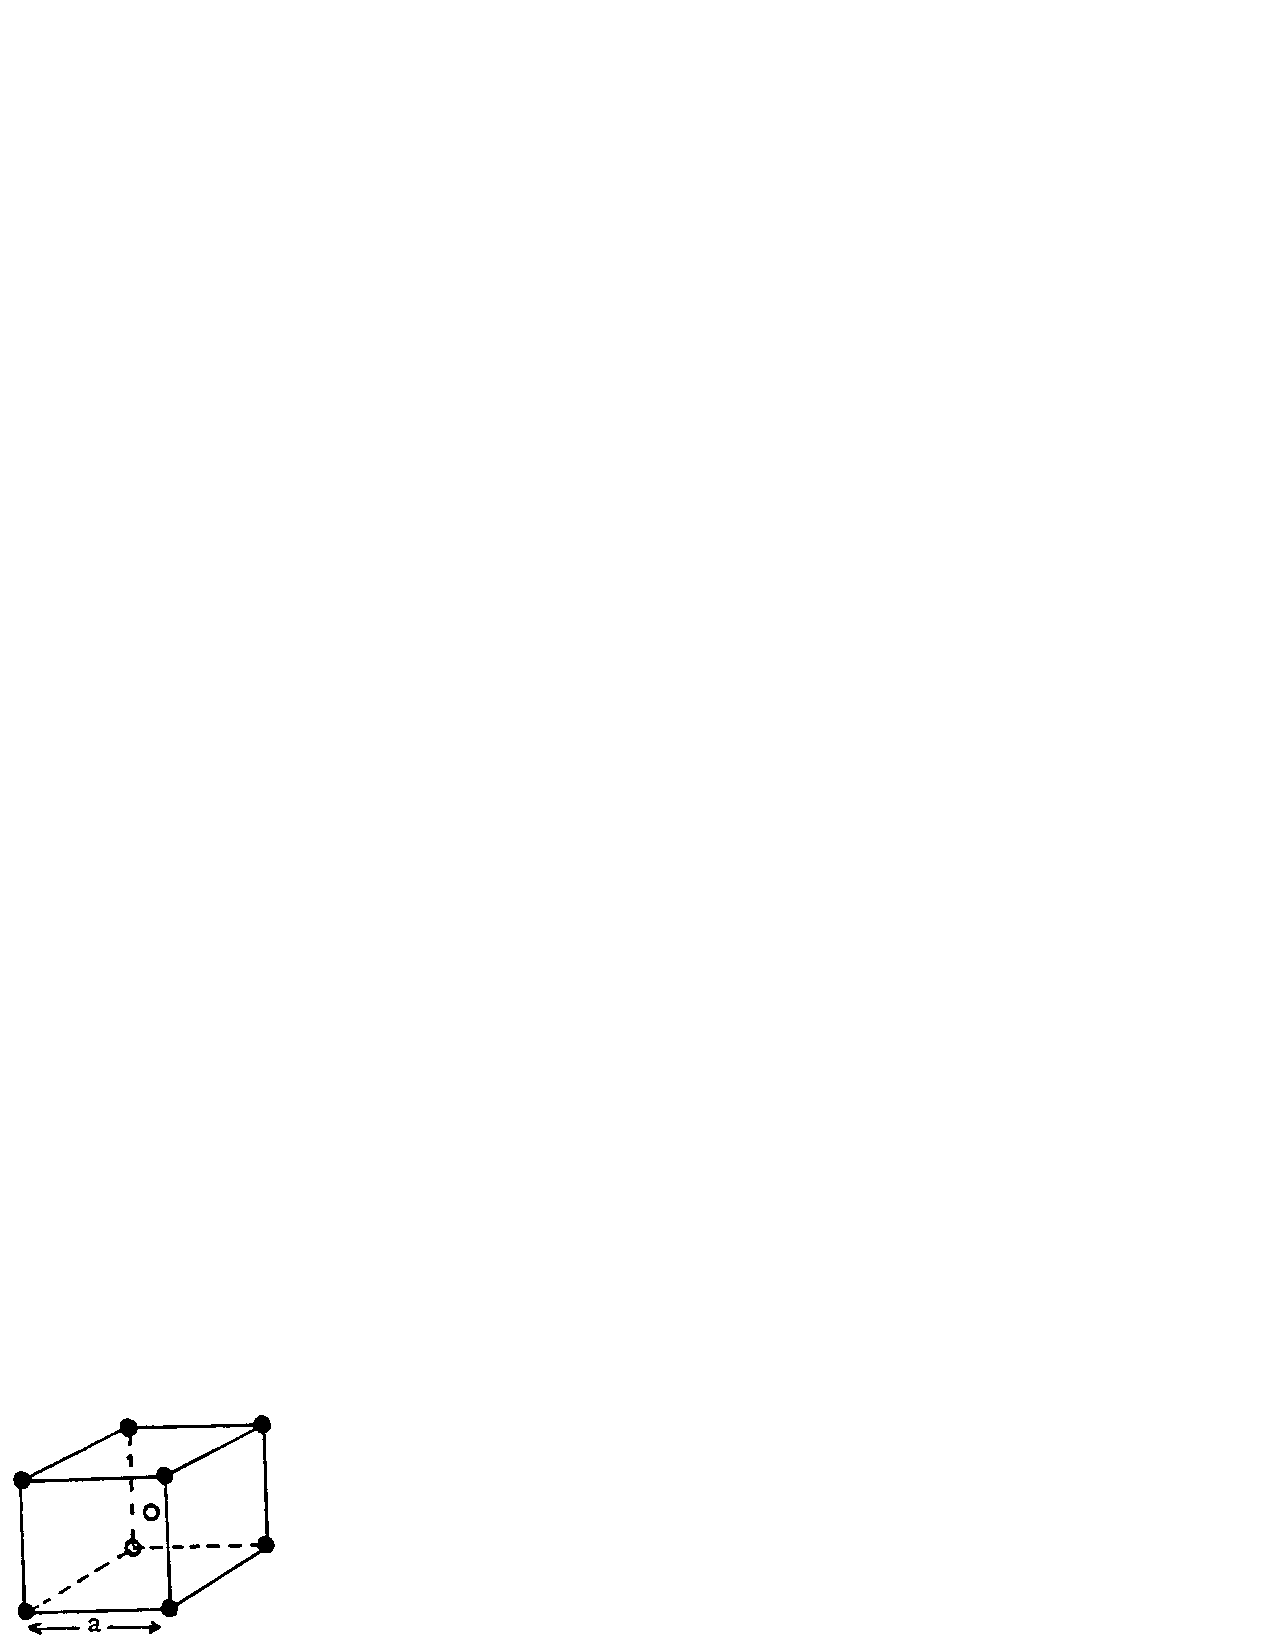
\includegraphics[scale=0.75]{fig14-02}
\caption{The body-centered cubic structure (type A2). 
Each atom has eight nearest neighbors at a distance of one-half
$\sqrt{3}a = 0.866$ a, where $a$ is the side of the cube, and six
second nearest neighbors at a.  Each of the eight corner atoms has
only one-eight of an atom inside the unit cube.  Thus, the total
number of atoms per cube is $1/8 \times 8 + 1 = 2$, and hence, the
volume per atom is one-half $a^3$.}
\label{chap14-fig1}
\end{figure}


\subsection{Face-centered Cubic (fcc)}

The face-centered cubic, fcc, structure consists of cubic unit cells,
such as in Figure \ref{chap14-fig2}, containing an atom at each corner
and at the center of each face.

\begin{figure}
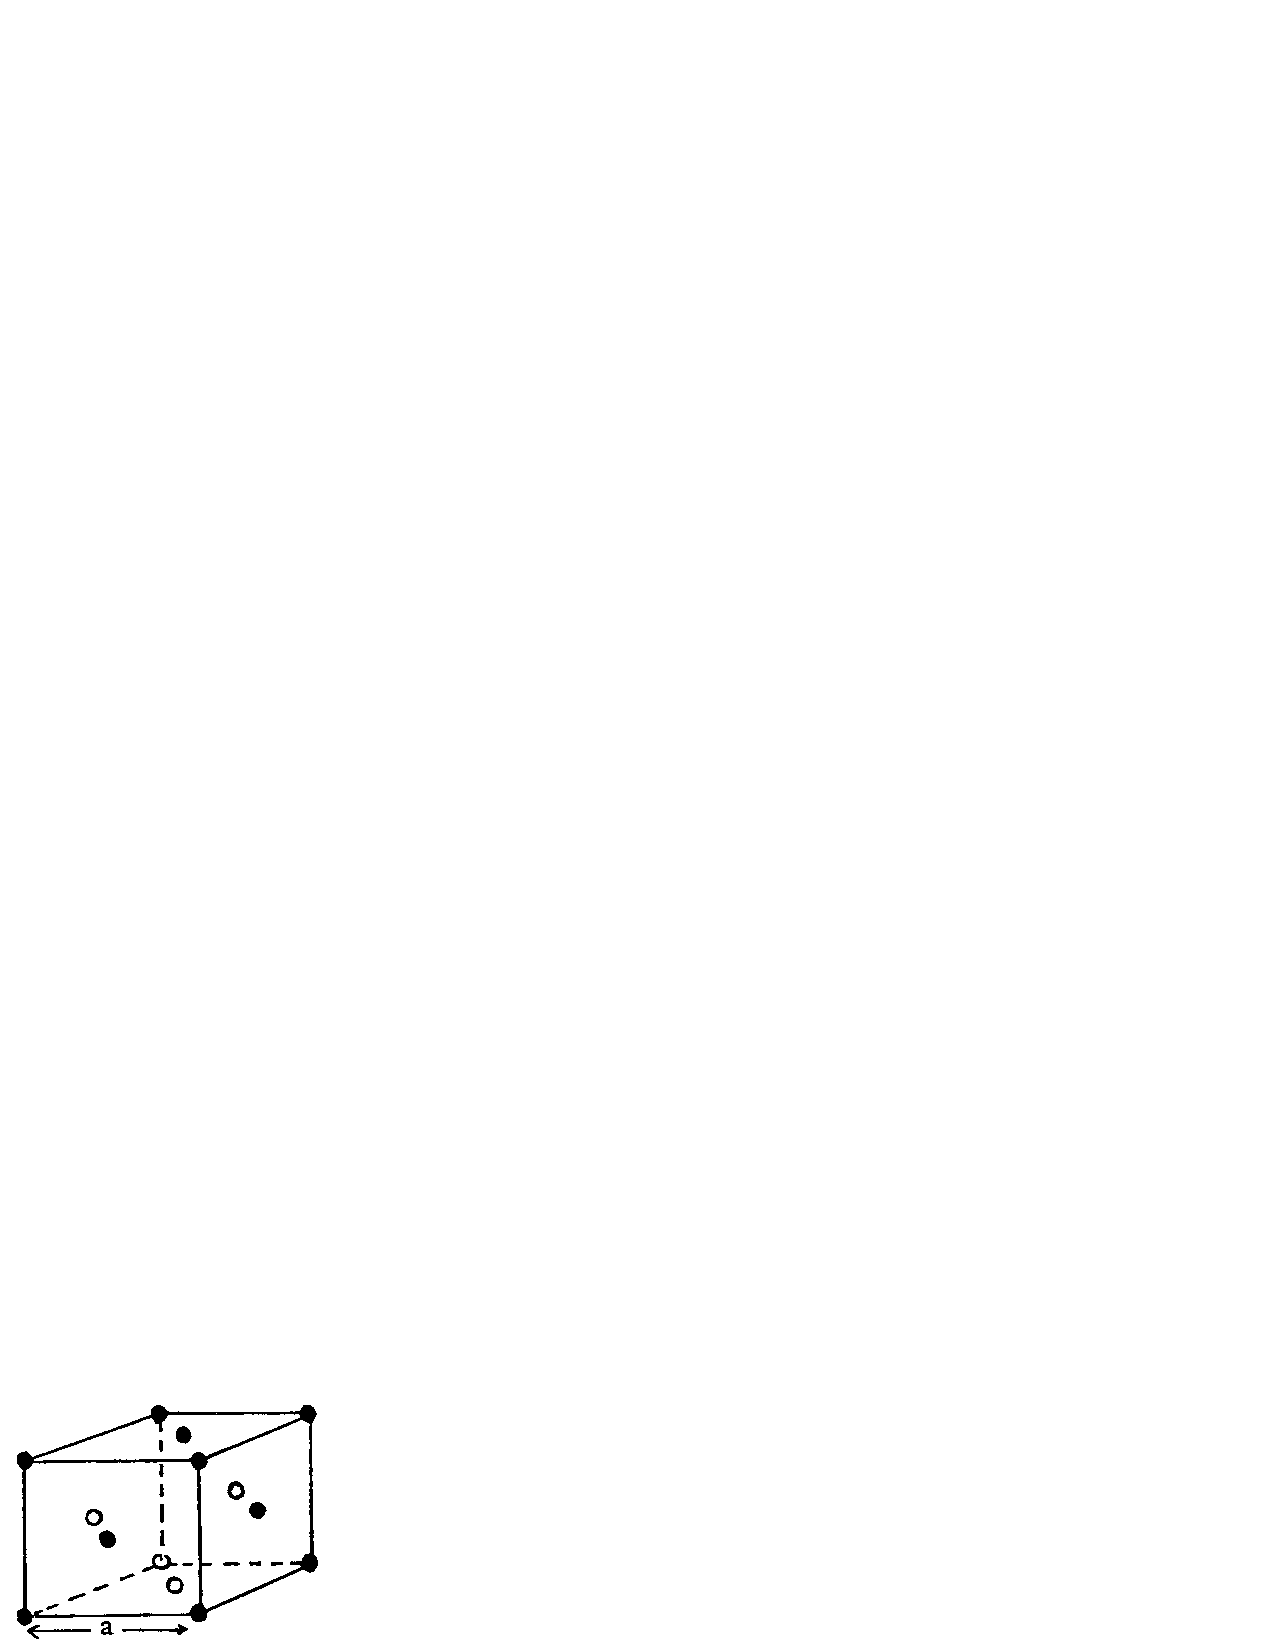
\includegraphics[scale=0.75]{fig14-03}
\caption{The face-centered cubic  struture (type A1).  These
cubes are placed together to fill all space.  Each atom has twelves
nearest neighbors at a distance of one-half $\sqrt{2} a = 0.707$a, and
six second nearest neighbors at a distance of a.  Each of six face
atoms has one-half of the atom inside the unit cell.  Thus, the total
number of atoms per cube is $1/8 * 8 + 1/2 * 6 = 4$, and hence, the
volume per atom is one-quarter $a^3$.  }
\label{chap14-fig2}
\end{figure}


An alternate view of this structure is obtained by looking parallel to
a body diagonal, as in Figure \ref{chap14-fig3}.  Each layer is
closest-packed, as discussed in the next section.

\begin{figure}
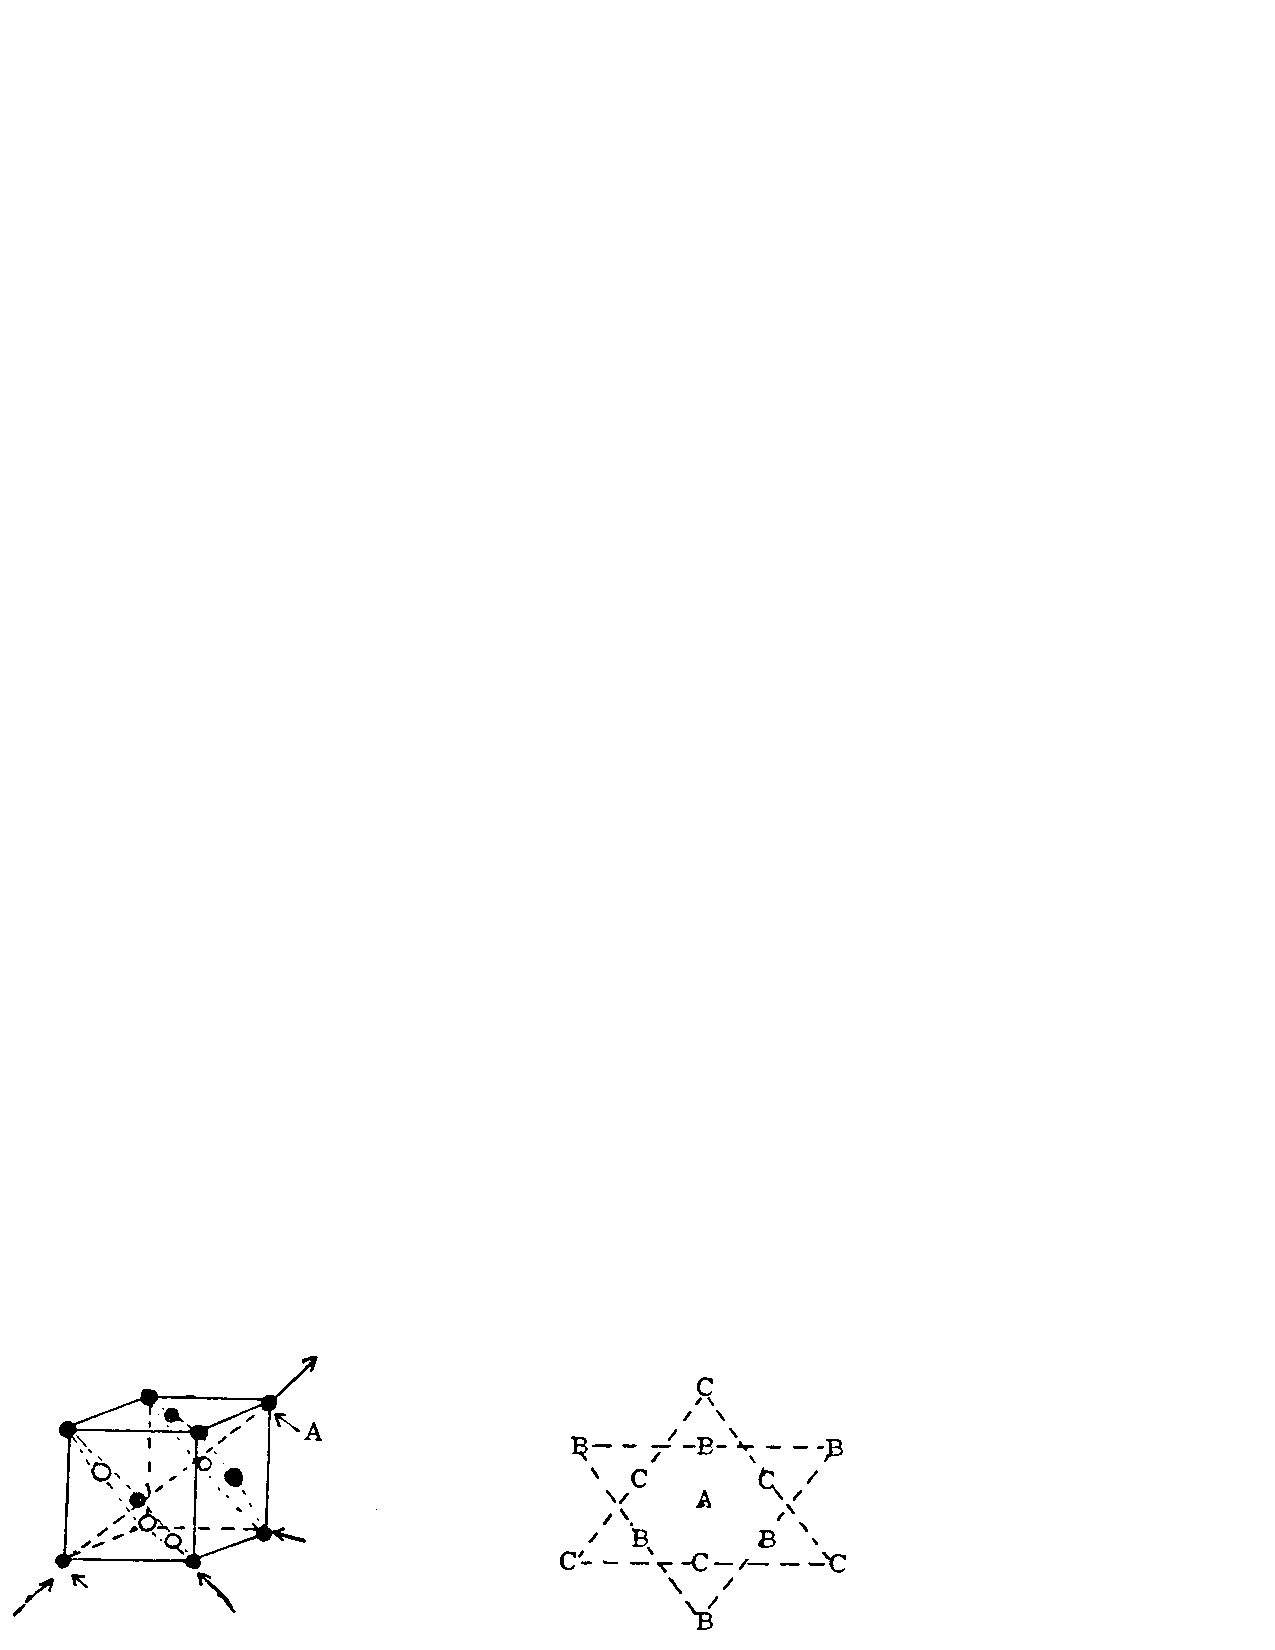
\includegraphics[scale=0.75]{fig14-04}
\caption{The closest-packed planes in the 
face-centered cubic structure. (b) is a view along the body diagonal
of (a).  The layers are separated by one-third $\sqrt{3}a = 0.577$a.}
\label{chap14-fig3}
\end{figure}

\subsection{Closest-Packed Structures}

A layer of atoms is closest-packed if each atom has six, equidistant,
nearest neighbors in the plane, as in Figure \ref{chap14-fig4}.  This
is the densest packing of equal sized spheres within a plane.
\begin{figure}
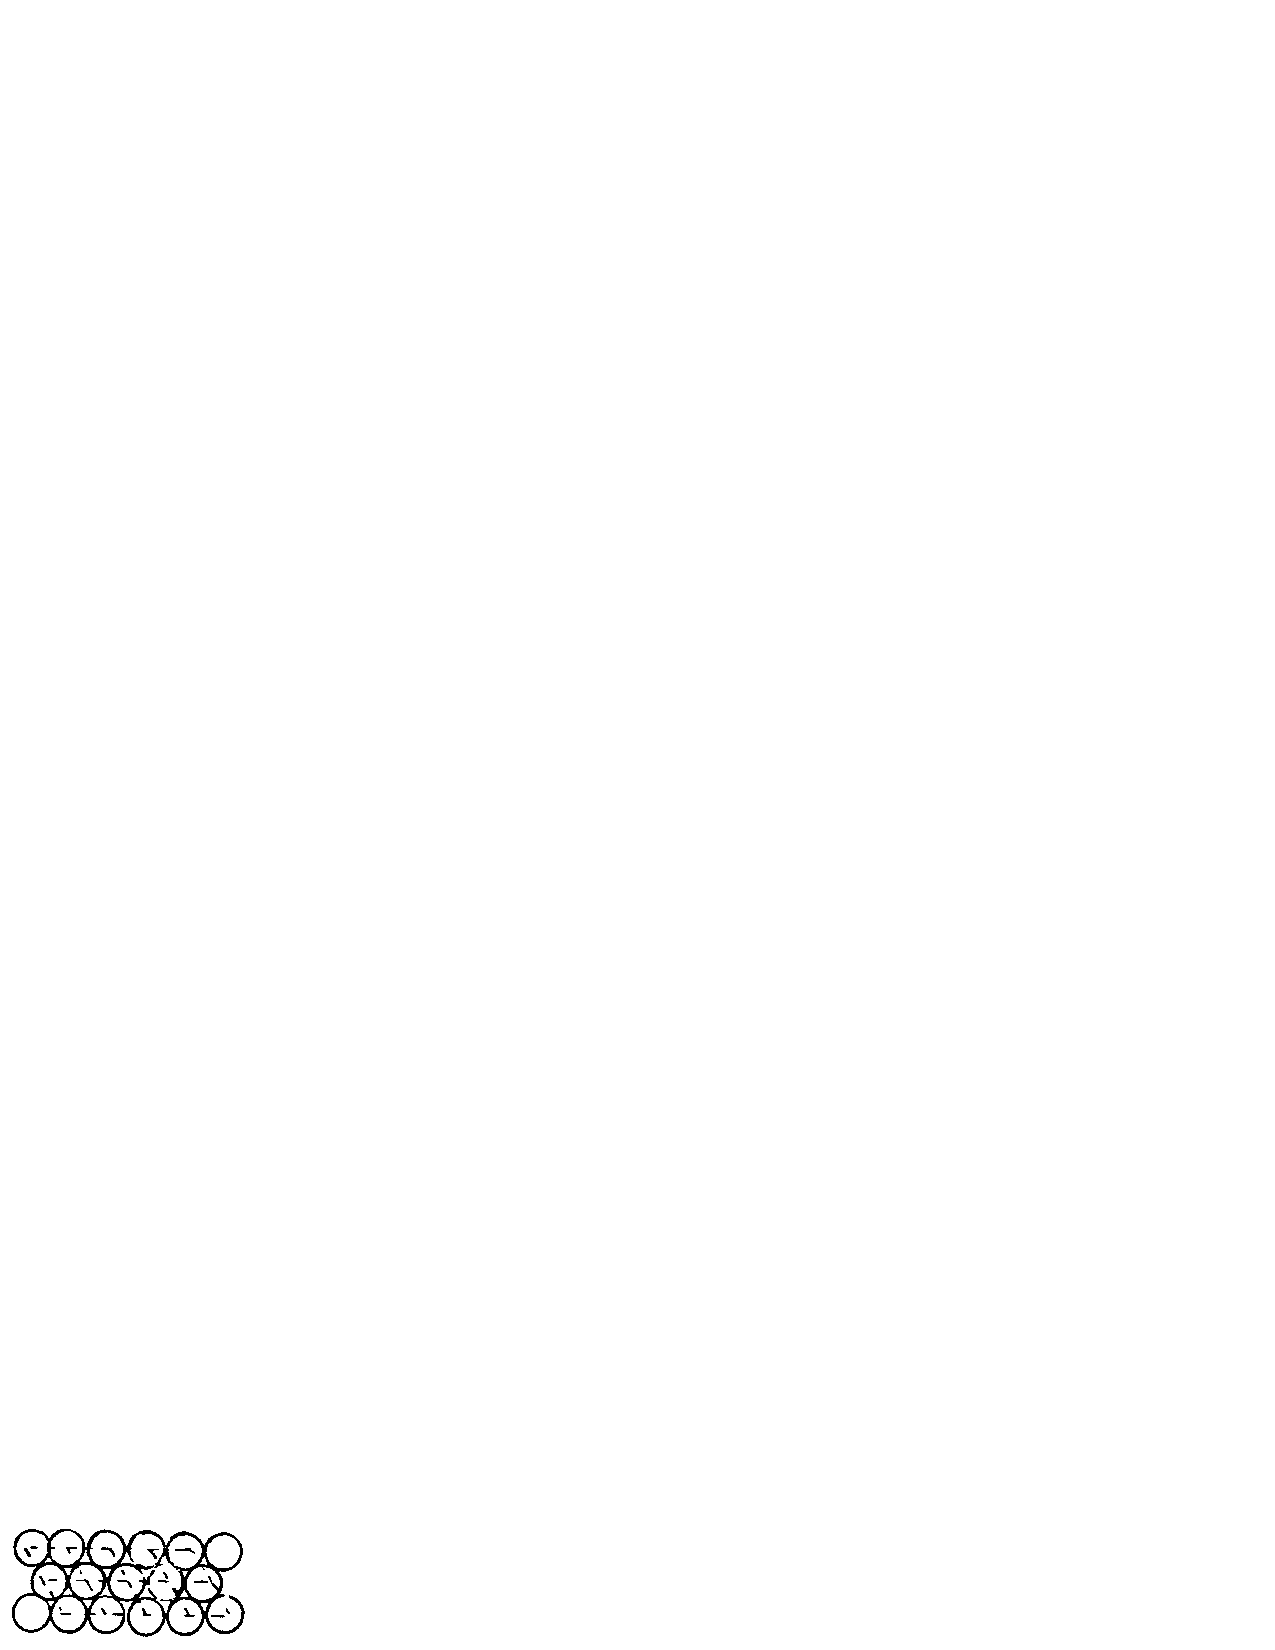
\includegraphics[scale=0.75]{fig14-05}
\caption{A closest-packed plane, illustrating the rhombic unit 
cells.  Such closest-packed layers may be stacked on top of each other
so that each atom of one layer touches three atoms of the layer above,
leading to twelve nearest neighbors.}
\label{chap14-fig4}
\end{figure}

There are two mutually exclusive ways of stacking any two layers as
indicated in Figure \ref{chap14-fig5}.
\begin{figure}
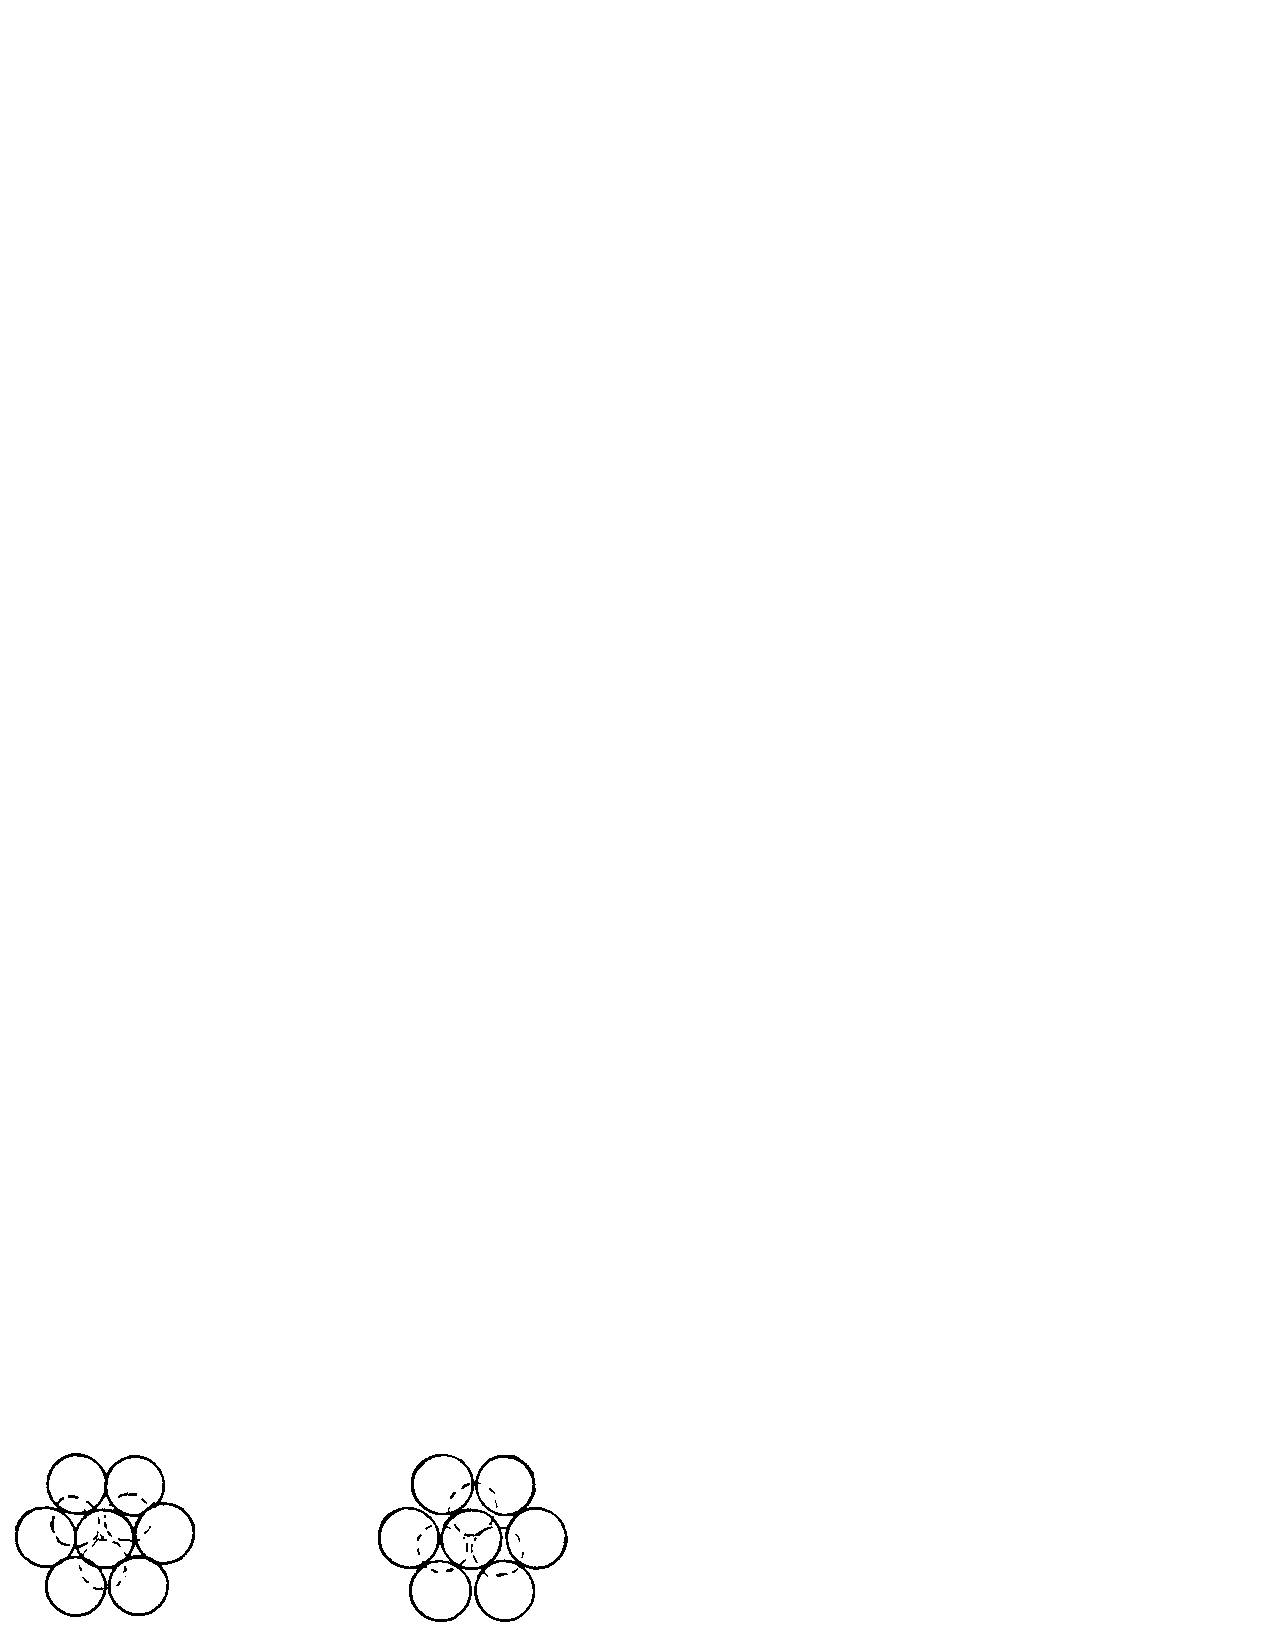
\includegraphics[scale=0.75]{fig14-06}
\caption{Stacking a new closest-packed layer on top of layer A.}
\label{chap14-fig5}
\end{figure}

The simplest periodic stacking of layers is thus ABABABABA so that the
third layer is directly above the first layer.  The three-dimensional
crystal structure resulting from this is referred to as
\emph{hexagonal closest-packed} (hcp).  The unit cell within a layer,
i.e., the smallest unit that can be translated periodically to fill
all space, is a rhombus as indicated in Figure \ref{chap14-fig4}.
Thus, the three-dimensional unit cell for hexagonal closest-packed is
the rhombic prism, as indicated in Figure \ref{chap14-fig5}, with
height $c$ and bottom side $a$, and included angle of 120$^{\circ}$,
and with two atoms per unit cell, one at the corner and one inside.

\begin{figure}
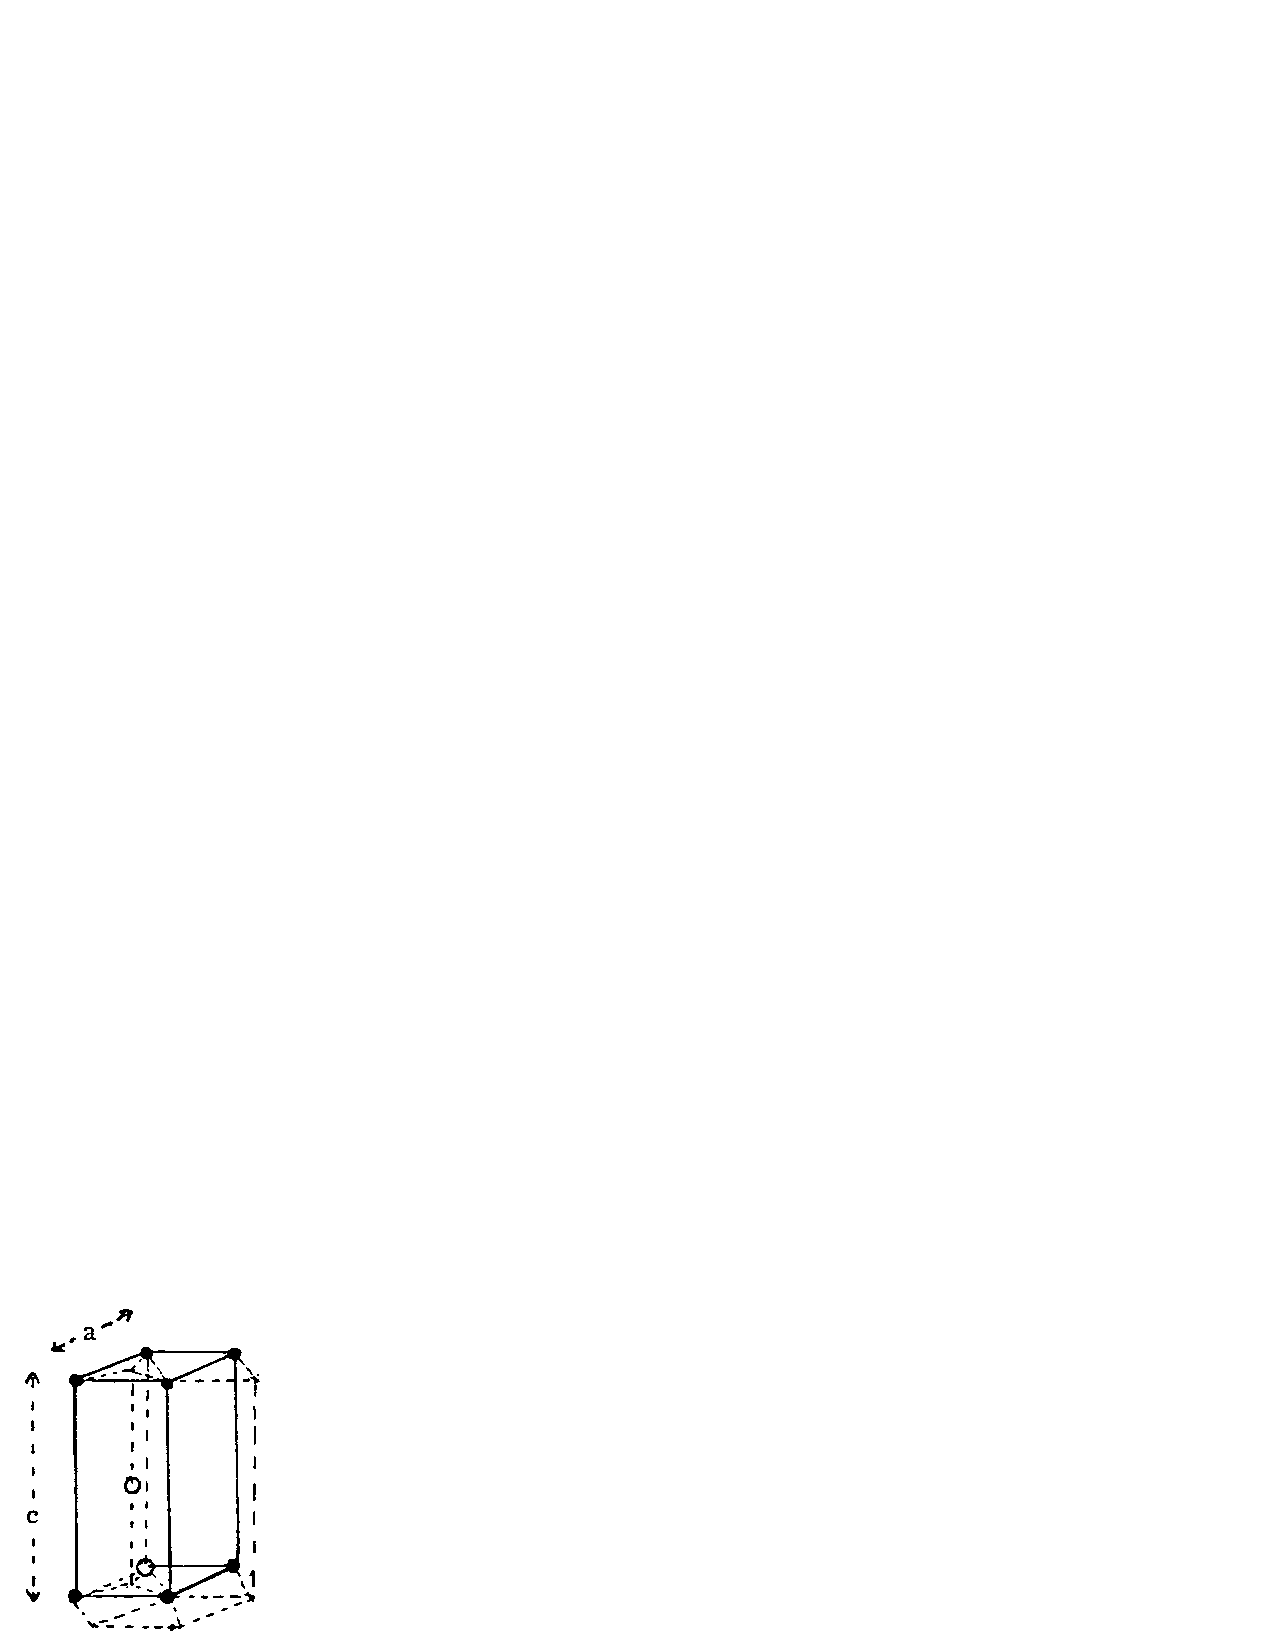
\includegraphics[scale=0.75]{fig14-07}
\caption{The unit cell for the hexagonal closest-packed structure (type A3).}
\label{chap14-fig6}
\end{figure}

For true closest
packing, twelve equidistant nearest neighbors with bond distance $R$, the 
distance between layers must be one-third $\sqrt{6}R$, and hence, $c = 
2/3 \sqrt{6}R$ while $a = R$, leading to
\begin{equation}
{c \over a} = {2 \over 3} \sqrt{6} = 1.633 .
\end{equation}
Assuming that you have forgotten your analytical geometry, this can be
calculated from Figure \ref{chap14-fig4} as follows.  The distance
between layers is
\begin{equation}
d_{layer} = {1 \over 3} \sqrt{3}a
\end{equation}
whereas, the bond distance is
\begin{equation}
R = {1 \over 2} \sqrt{2} a.
\end{equation}
Thus,
\begin{equation}
{d_{layer} \over R} = \sqrt{{2 \over 3}} = 0.8165 .
\end{equation}
For hexagonal closest-packed
\begin{equation}
{c \over a} = {2d_{layer} \over R} = 1.6330.
\end{equation}
Some systems lead to values close to this, e. g., for Mg $c/a = 
1.624$, whereas others deviate significantly, e.g., for Zn $c/a = 1.856$.

A second way to stack the layers is ABCABCABC so that the first and
fourth layers are equivalent.  Careful examination of Figure
\ref{chap14-fig3} shows that this stacking in equation
(\ref{chap14-eqno2}) is exactly equivalent to that along the diagonal
of the face-centered cubic structure. For this reason, face-centered
cubic is often referred to as cubic closest-packed, ccp.

A third common stacking is ABACABAC
This is-referred to as double hexagonal closest-packed, or 
2-hexagonoal closest-packed, and is exhibited by the lighter 
lanthanides, or rare earths, and heavier actinides, or transuranics.

\section{The Li and Cu Columns}

\subsection{The Alkali Metals, Li Column}

For Li, Na, K, Rb, and Cs, the stable crystalline form at room
temperature is body-centered cubic, bcc.  For Li and Na the
equilibrium structure is hexagonoal closest-packed at low temperature,
T $< 720^{\circ}$ K for Li and T $< 36^{\circ}$ K for Na.  For Li, a
face-centered cubic phase has also been observed after cold working,
at T $< 78^{\circ}$K, but not in Na.  For K, Rb and Cs no transitions
were observed down to 5$^{\circ}$K, even upon cold working.  The bond
distances for different phases are compared in Table
\ref{chap14-tab2a}, where we see that face-centered cubic and
hexagonal closest-packed lead to nearly identical bond distances but,
that body-centered cubic has a shorter bond distance.

\begin{table}
\caption{Bond distances of alkali atoms for different phases.}
\label{chap14-tab2a}
\begin{tabular}{ccc}\\ \hline
& Li & Na\cr
& (78$^{\circ}$ K& (5$^{\circ}$ K\cr
\noalign{\medskip\hrule\medskip}
body-centered cubic & 3.016 & 3.658\cr
hexagonal closest-packed & 3.103, 3.108 & 3.767, 3.768\cr
face-centered cubic & 3.103\cr
\hline
\end{tabular}
\end{table}

\begin{table}
\caption{Bond distances of alkali, body-centered cubic, and 
noble, face-centered cubic, metals.}
\label{chap14-tab2b}
\begin{tabular}{ccccc}\\ \hline
&\multicolumn{2}{c}{Solid}&\multicolumn{2}{c}{Diatomic}\cr
& 5$^{\circ}$ K & 20$^{\circ}$  C & $M^+_2$ & $M_2$\cr 

Li & 3.014 & 3.039 & 3.127$^a$ & 2.67\cr
Na & 3.659 & 3.716 & (3.54) & 3.08\cr
K & 4.525 & 4.608 & (4.11) & 3.91\cr
Rb & 4.837 & 4.936 & (3.94)\cr
Cs & 5.235 & 5.349 & & 4.47\cr
Cu & & (3.6148) & & 2.22\cr
Ag & & (4.0857)\cr
Au & & 4.0782 & & 2.47\cr
\hline
\end{tabular}\\
$^a$ Konowalow, theory.
\end{table}

\begin{table}
\caption{Thermodynamic porperties of the monovalent metals.}
\label{chap14-tab2c}
\begin{tabular}{ccccccc}\\ \hline
&\multicolumn{3}{c}{Bond Energy Per Electron$^c$}
&\multicolumn{3}{c}{Properties Solid}\cr
Structure & $M_2$ & $M^+_2$ & Solid$^a$ & $T_{mp}$ & $\Delta H_m$ & 
$T_{bp}$\cr
& & & & ($^{\circ}$K) & (kcal) & ($^{\circ}$K)\cr

Li bcc & 12.1 & 33.7 & 37.7	& 453.7 & 0.717 & 1615\cr
Na bcc & 8.3 & 22.1 & 25.66 & 371.0 & 0.621 & 1156\cr
K bcc & 5.9 & 19.6 & 21.54 & 336.4 & 0.558 & 1032\cr
Rb bcc & 5.7 & $\geq$16. 6 & 19.64 & 312.6 & 0.524 & 961\cr
Cs bcc & 4.5 & 14.1 & 18.54 & 301.55 & 0.500 & 944\cr
Cu fcc & 23.8 & 54.96 & 80.2 & 1356.6 & 3.12 & 2836\cr
Ag fcc & 19.2 & & 67.8 & 1234 & 2.7 & 2436\cr
Au fcc & 26.5 & & 88.0 & 1336.15 & 3.0 & 3130\cr
\hline
\end{tabular}\\
$^a$ Reference 2, 0$^{\circ}$ K.
$^b$ References 4s, 20$^{\circ}$ C.
$^c$ In kcal.
\end{table}

In order for the volume per atom to be equal for body-centered cubic and 
face-centered cubic structures, we require
\begin{equation}
{1 \over 2} a^3_{bcc} = {1 \over 4} a^3_{fcc}
\end{equation}
or
\begin{equation}
{a_{fcc} \over a_{bcc}} = (2)^{{1 \over 3}} = 1.260 .
\end{equation}
Thus, since
\begin{equation}
R_{bcc} = {1 \over 2} \sqrt{3} a_{bcc}
\end{equation}
and
\begin{equation}
R_{fcc} = {1 \over 2} \sqrt{2} a_{fcc},
\end{equation}
we obtain
\begin{equation}
{R_{fcc} \over R_{bcc}} = {\sqrt{2} \over \sqrt{3}} {a_{fcc} \over 
a_{bcc}} = \sqrt{{2 \over 3}} {a_{fcc} \over a_{bcc}} = 1.029
\label{chap14-eqno4}
\end{equation}
for the case of equal volumes.  The values observed for Li and Na are both 
1.030, in excellent agreement with the equal volume assumption.

With one valence electron per atom, one can clearly not make normal 
covalent bonds between all near-neighbor atoms.  The generally accepted 
view is in terms of the molecular orbitals spread over the entire infinite 
crystal. Starting with the $3s$ orbital of Na on each of the
N atoms of the crystal, $N \sim 10^{22}$, this would lead to $N$ 
molecular orbitals spread over some energy range, the $3s$ band, and 
similarly for the $3p$.  For normal internuclear distances there is
essentially a continuum of levels, referred to as the conduction band. 
With $N$ electrons we need only occupy the lowest $N/2$ orbitals to get 
the ground state.  There are numerous states
infinitely close to the ground state and hence, small electric fields can 
generate an electrical current.  Thus, such systems are expected to be
metals.

\begin{figure}
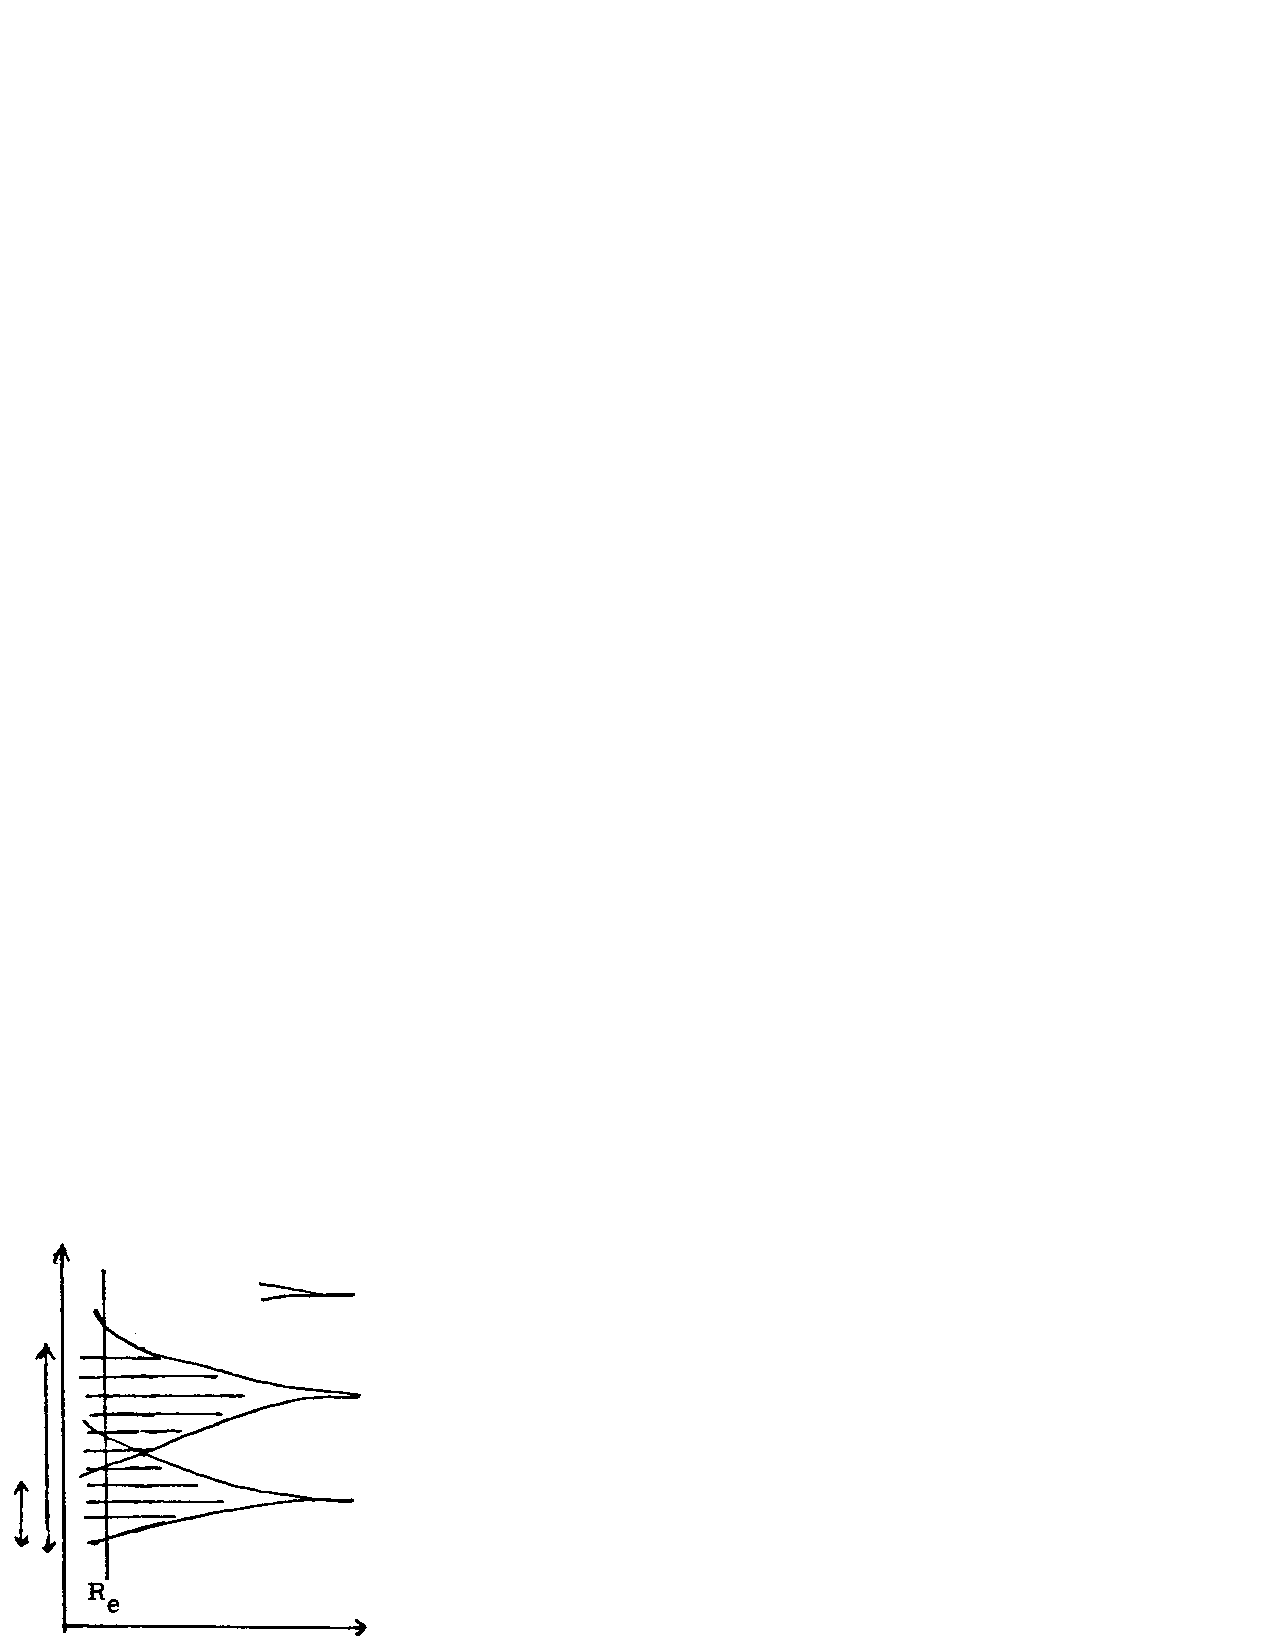
\includegraphics[scale=0.75]{fig14-08}
\caption{The separation of energy levels for a metal.  Unfortunately,
such a picture does not allow us to make qualitative analyses of why
Na has the body-centered cubic structure while Cu has face-centered
cubic, or why numerous other structures are not as good.}
\label{chap14-fig7}
\end{figure}

Pauling suggested a valence bond view of such metals involving
configurations with one bond pair between specific atoms as
illustrated in Figure \ref{chap14-fig8}, but with a superposition, or
resonance, of all possible such structures.  This is referred to as
the \emph{resonating valence bond} model of metals.  Unfortunately,
this picture does not yield a qualitative analysis of structure.

\begin{figure}
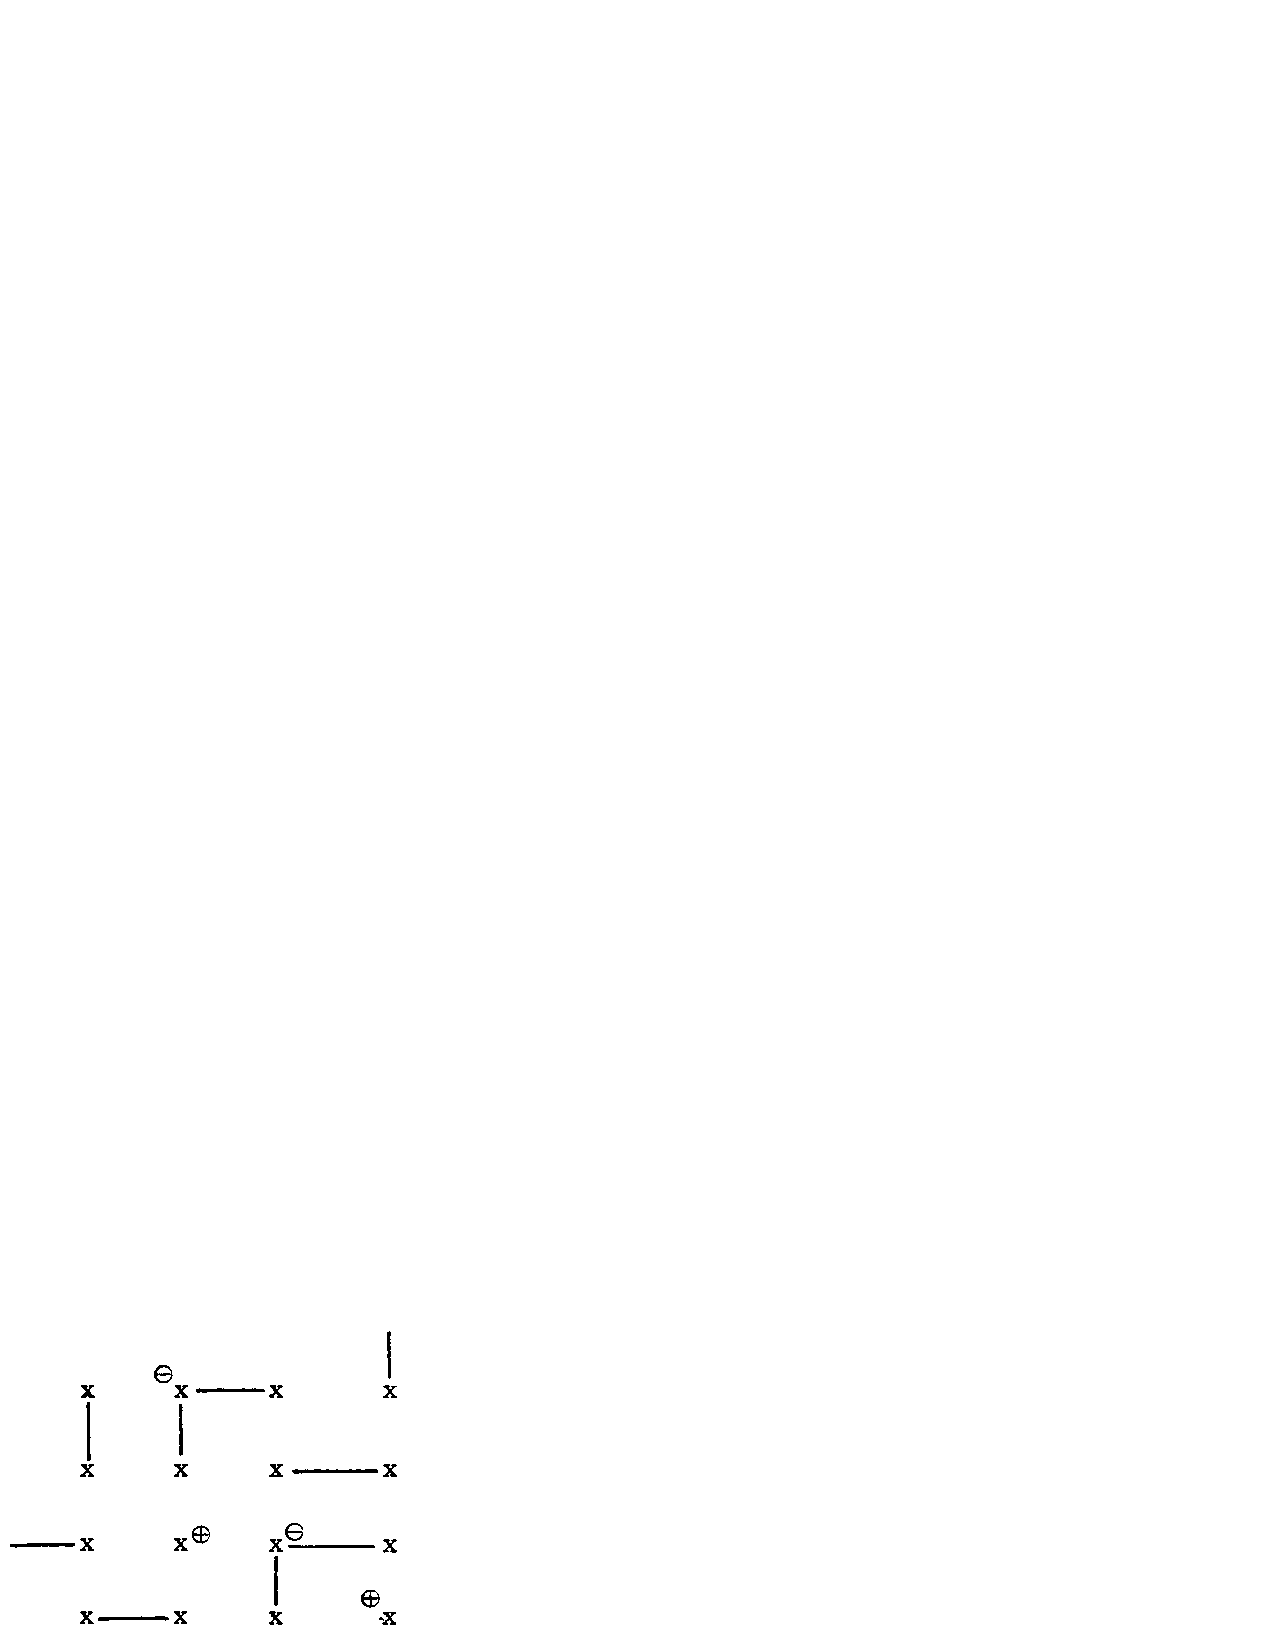
\includegraphics[scale=0.75]{fig14-09}
\caption{Pauling's resonating valence bond model of metallic bonding.}
\label{chap14-fig8}
\end{figure}

An alternative view, speculatively suggested in the Chemistry 120
course over the last decade, is based on the following observations.
For Na$^+_2$ the bond is 22.1 kcal per electron, while for Na$_2$ the
bond is 16.6/2 = 8.3 kcal per electron.  Thus, rather than making
two-electron bonds in the solid, we should make one-electron bonds
localized in different regions and coupled into singlet pairs,
$(\phi_a \phi_b + \phi_b \phi_a)(\alpha \beta - \beta
\alpha)$.  Indeed, studies$^1$ of the ground states of planar arrays of 
alkali atoms, Li$_n$ and Na$_n$ with $n = 3$ to 10, suggests that the
lowest state for planar systems is closest-packed with singly-occupied
orbitals localized in alternate triangles as indicated in Figure
\ref{chap14-fig9}.  These orbitals can be paired together in various
ways, only one of which is shown in the figure.  However, since the
overlaps are small, $S = 0.32$, the model of coupling is not critical
and resonance energies are small.

For three dimensions the speculation is that there are one-electron bonds 
centered in tetrahedron or octahedron paired together.

The correlations in Tables \ref{chap14-tab2a}--\ref{chap14-tab2c} for
the alkali metals, are consistent with such a description.$^{2,3}$
Thus, for example, the bond distance, 3.66 \AA, in solid Na is close
to that of Na$^+_2$, 3.54 \AA, but not to that of Na$_2$, 3.08 \AA.
Also shown in these tables are the melting temperature, $T_{mp}$, the
heat of fusion, $\Delta H_m$, and the boiling temperature, $T_{bp}$,
the temperature where the vapor pressure is 1 atm.

\begin{figure}
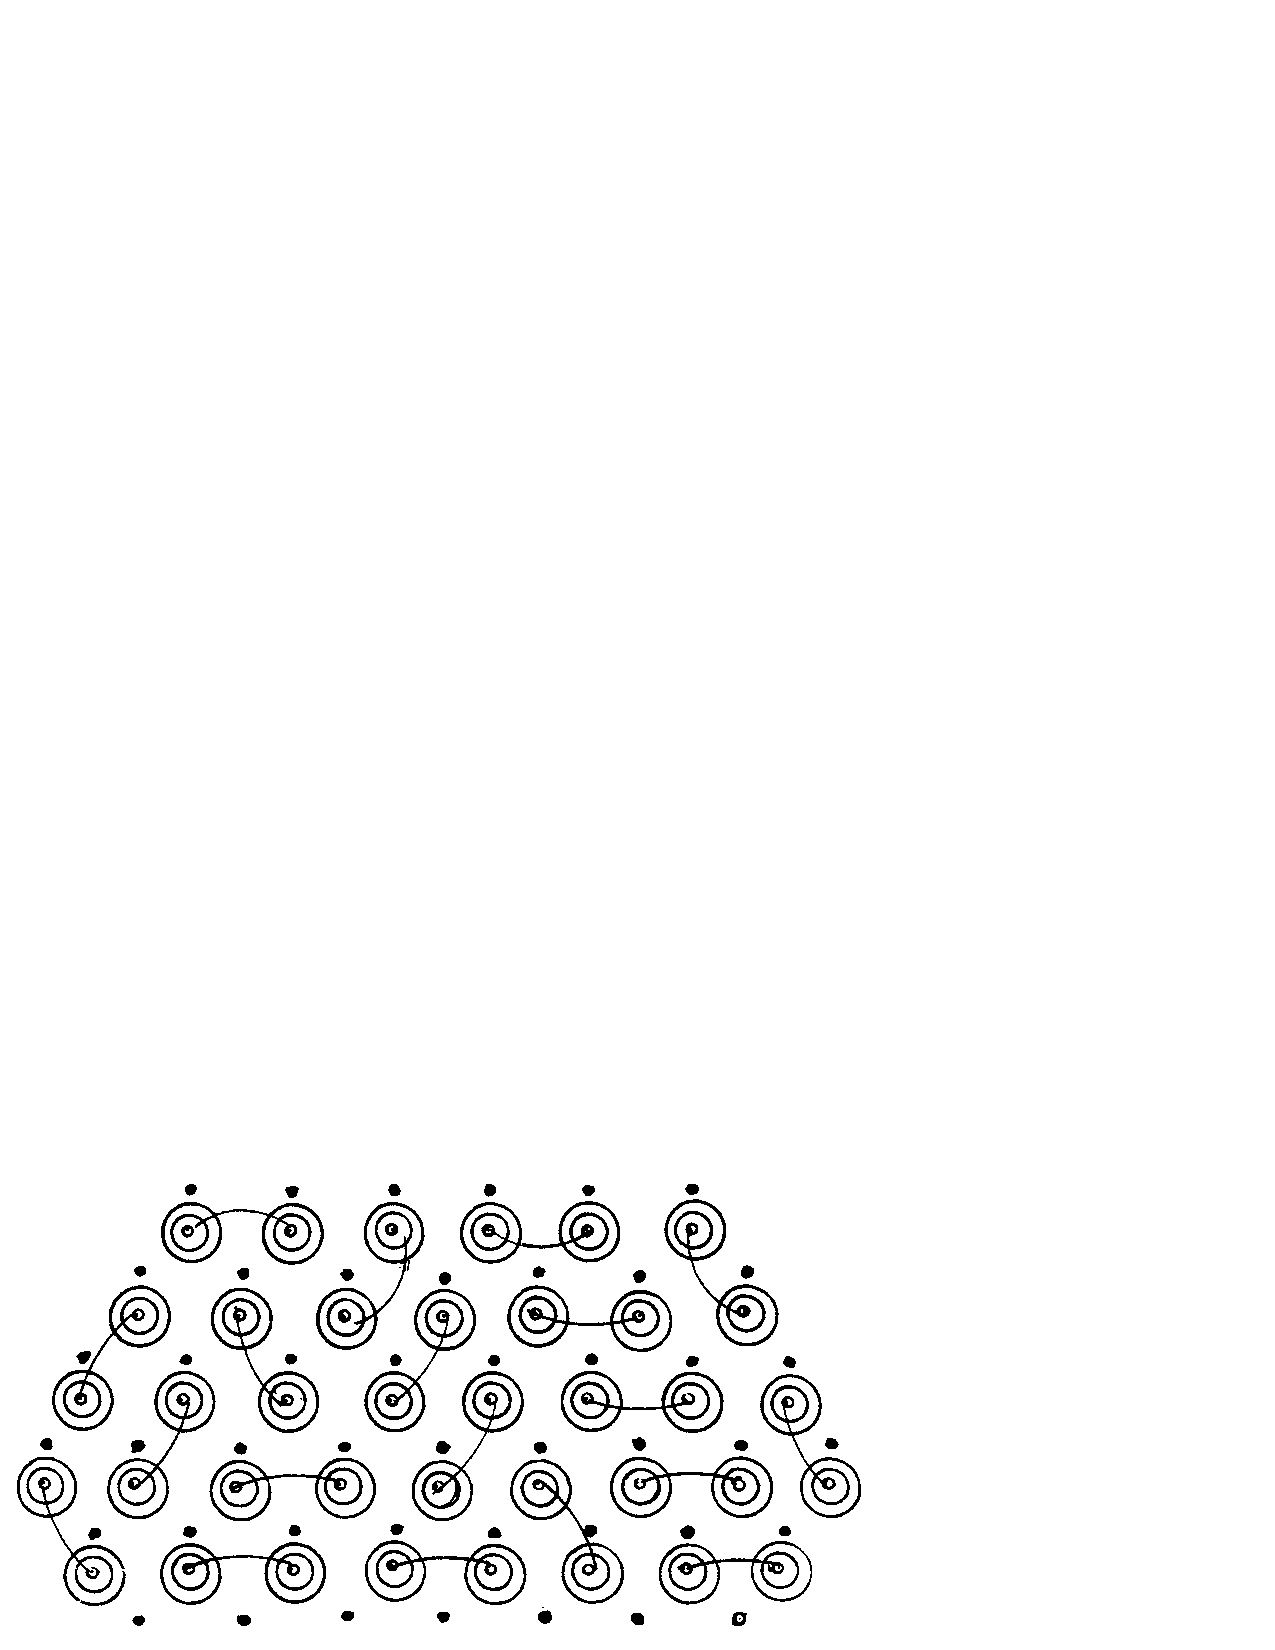
\includegraphics[scale=0.75]{fig14-10}
\caption{One-electron bond model of metallic bonding.}
\label{chap14-fig9}
\end{figure}

\subsection{The Noble Metals, Cu Column}

For noble metals such as Cu, Ag, and Au, the stable crystalline format
is face-centered cubic for all observed temperatures.  The properties
of these metals are given in Tables
\ref{chap14-tab2a}--\ref{chap14-tab2b}.  Despite the fact that the
alkali and noble metals have one valence electron per atom, there is
no comparison in the properties of these metals. The crystal structure
is different and the cohesive energy of the noble metals is far
higher.

Electrolytic deposition of metal films has led to metastable hexagonal 
closest-packed structures for Cu and Hg, and probably Au.  Within 
experimental error bond distances for hexagonal closest-packed Cu and 
Ag are equal to those for face-centered cubic.

\section{The Be and Zn Columns}

At room temperature, Be and Mg are hexagonal closest-packed, Ca and Sr are 
face-centered cubic, and Ba and Ra are body-centered cubic. So
much for the periodic table!  For Be, Ca, and Sr there is a transformation to 
body-centered cubic at high temperature.

For Zn and Cd the hexagonal closest-packed structure is stable at all 
temperatures but leads to a severe distortion in which the atoms within 
a closest-packed plane are squeezed together relative to the
atoms above and below the plane.  Hg crystallizes in a rhombohedral unit 
cell, A10, which can be visualized as a distorted face-centered cubic in 
which the bonds within a closest-packed plane are stretched to
3.465 \AA\ at 78$^{\circ}$K, while the six neighbors above and below the 
plane remain at 2.993 \AA.  Thus, Hg differs markedly from Zn and Cd.

In the valence bond description, formation of Mg$_2$ involves one new bond pair
\begin{equation}
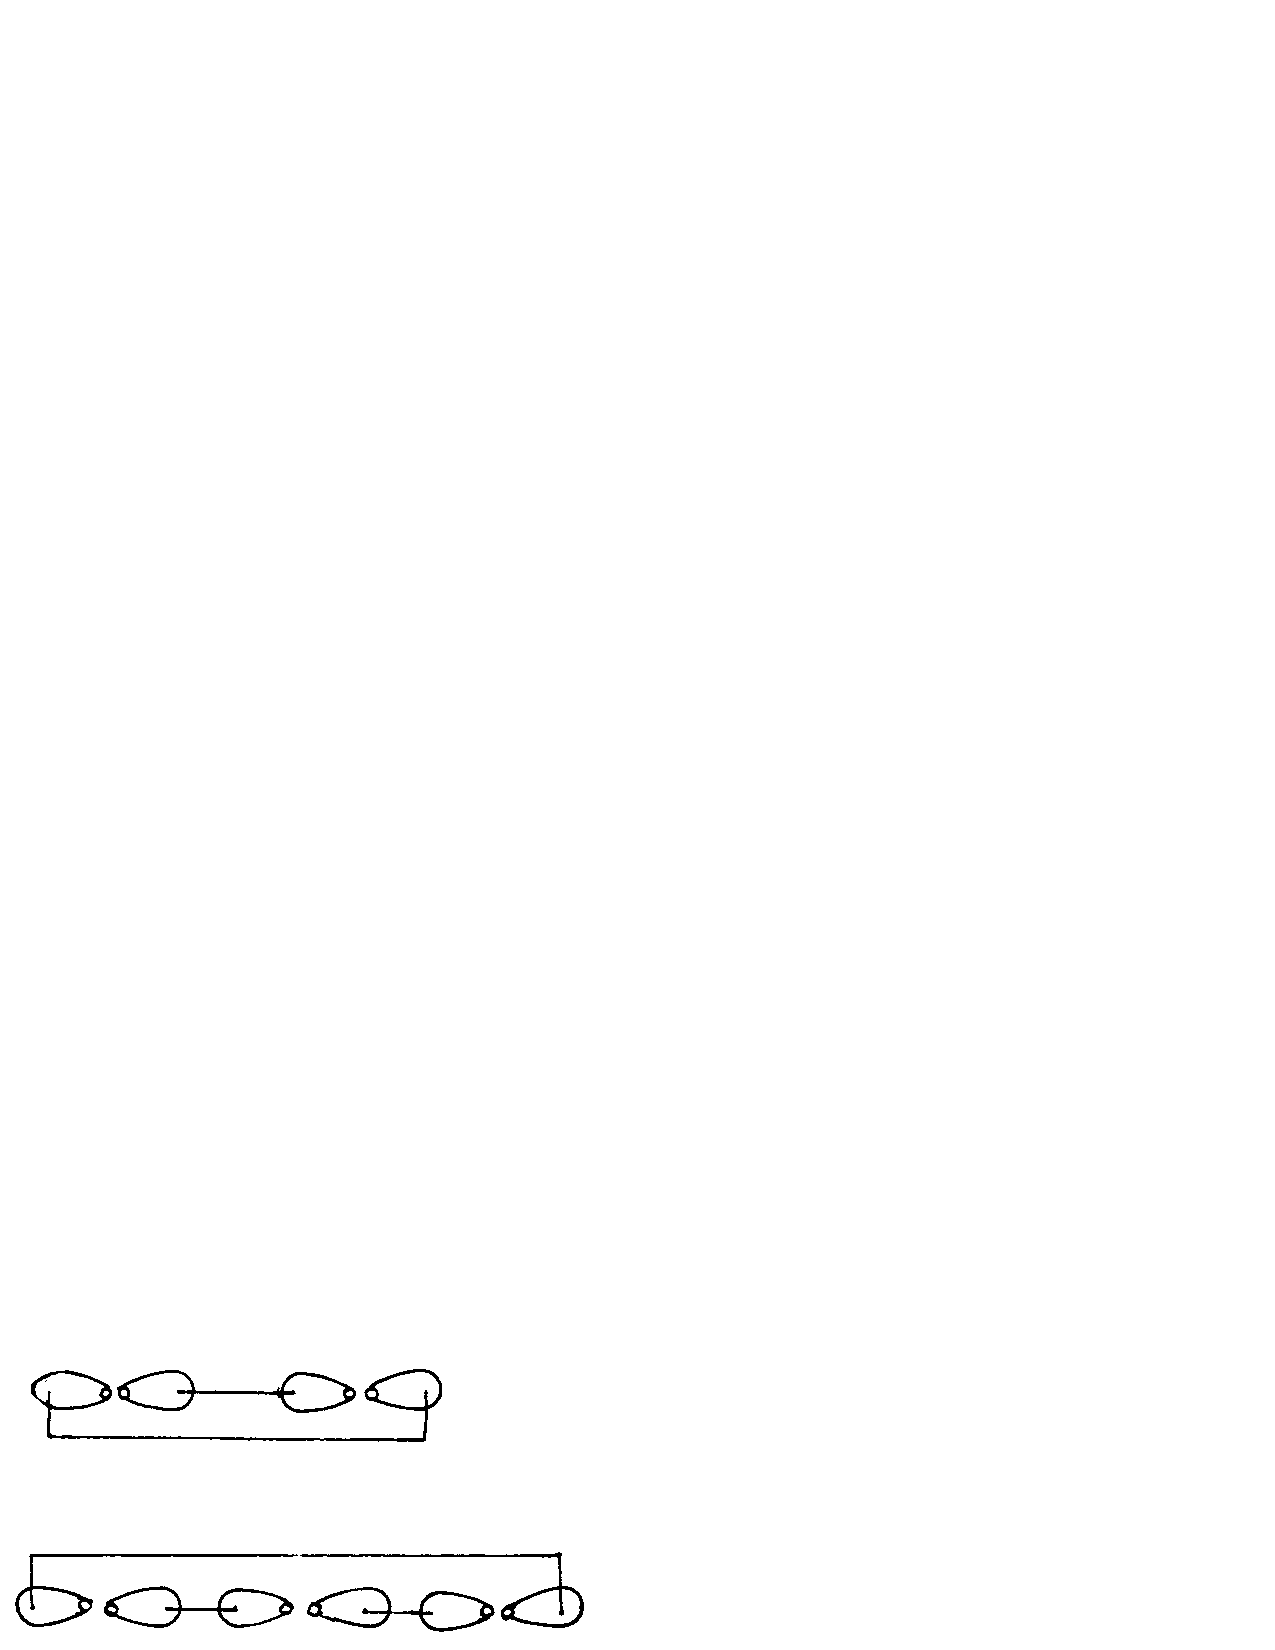
\includegraphics{fig14-10a}
\end{equation}
and one antibond.  Bonding three Mg atoms together leads to
\begin{equation}
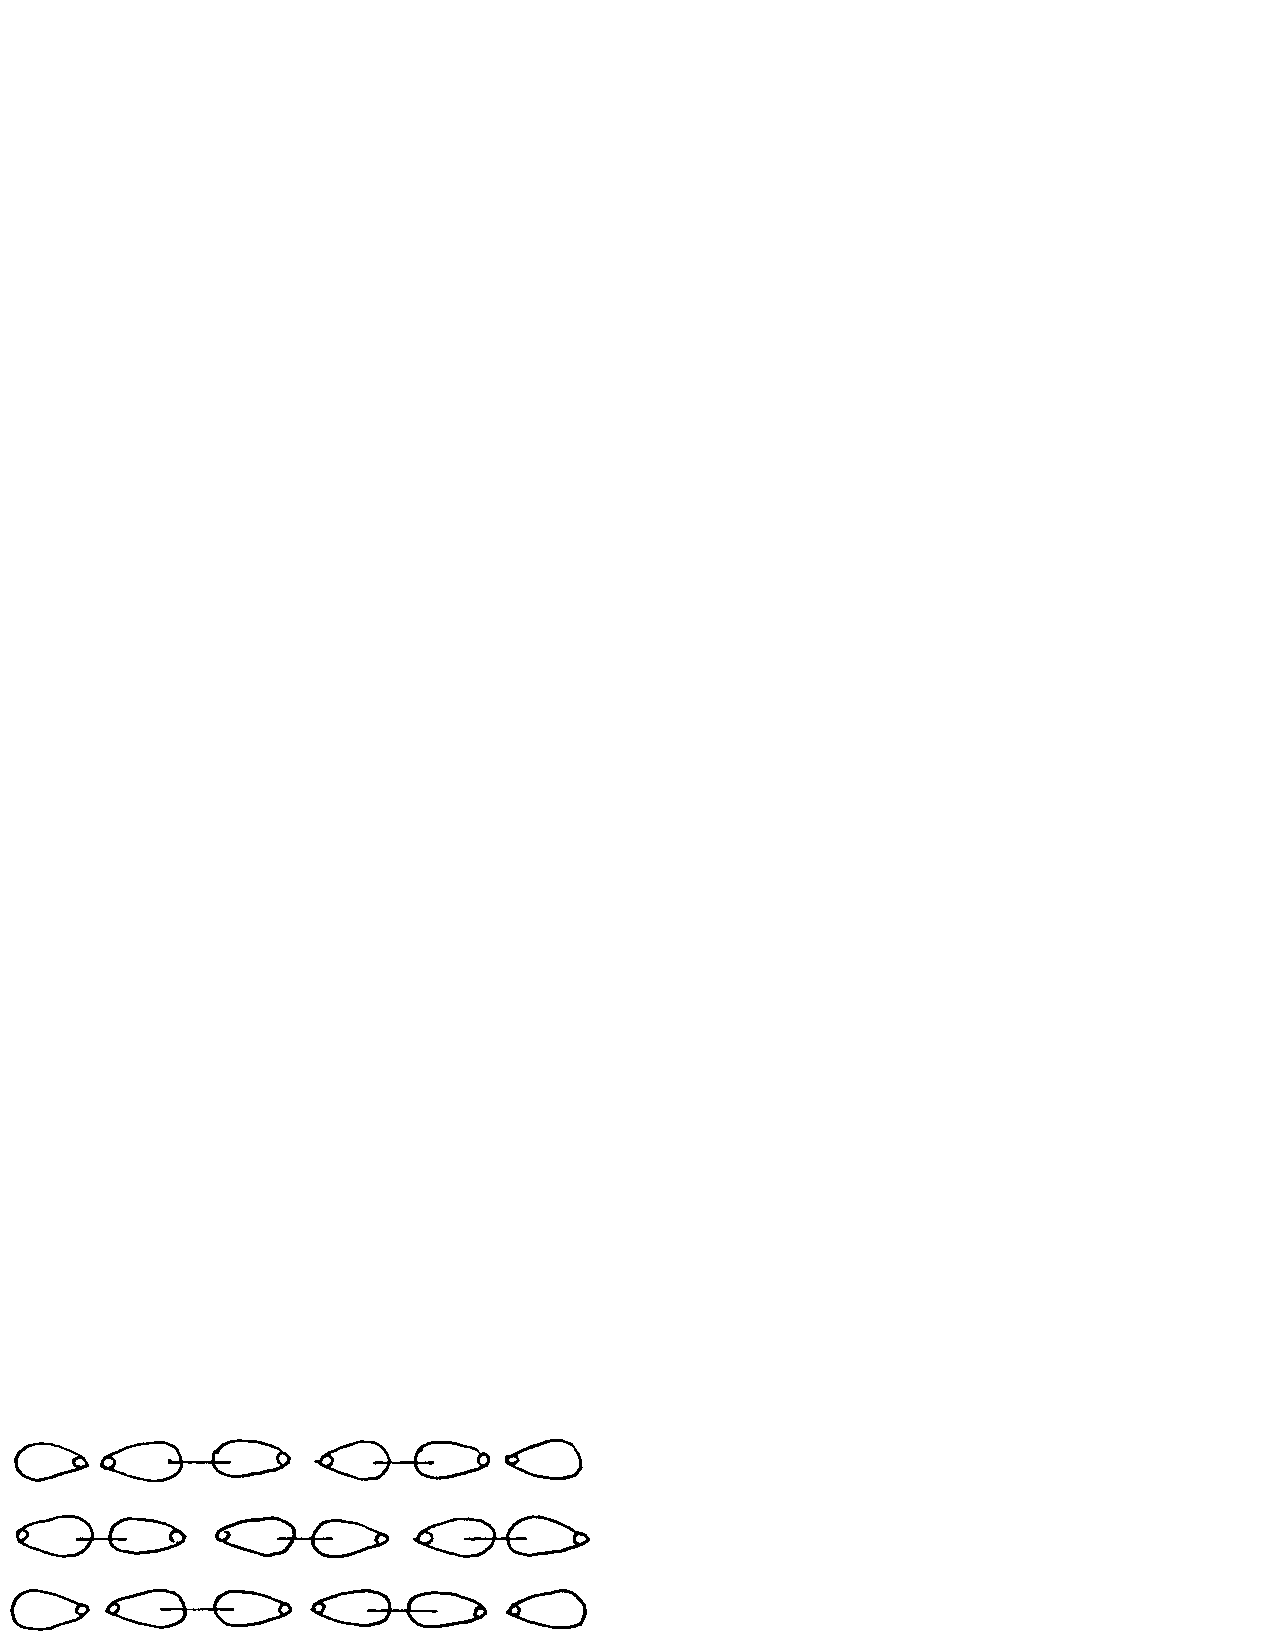
\includegraphics{fig14-10b}
\label{chap14-eqno5}
\end{equation}
Thus, we get two bond pairs and one antibond with smaller overlap.  Hence, 
even though the dimer Mg$_2$ is not strongly bound, it seems likely that 
larger chains will have greater stability.

In equation (\ref{chap14-eqno5}) we have left the $p_x$ and $p_y$
orbitals empty, taking the axis as $z$.  Thus, collections of such
chains might prefer to be staggered so that the electron pair in one
chain is close to the nuclei of adjacent chains as in equation
(\ref{chap14-eqno6})
\begin{equation}
% missing figure
%
\includegraphics{fig14-10c}
\label{chap14-eqno6}
\end{equation}
This leads to a net of the form
\begin{equation}
% missing figure
%\includegraphics{fig14-10d}
\label{chap14-eqno7}
\end{equation}
With equal separations, this net allows a description such as equation
(\ref{chap14-eqno6}) in three directions within the plane, leading to
a closest-packed layer.

Since the lower temperature forms of all these elements involve
closest-packed planes, the bonding might be similar to that implied by
equation (\ref{chap14-eqno6}).  A special problem is to explain why
Zn, Cd, and Hg are so distorted.

In the molecular orbital or band model, there are $2N$ electrons to
place in the lowest $N$ molecular orbitals, see Figure
\ref{chap14-fig10}.

\begin{figure}
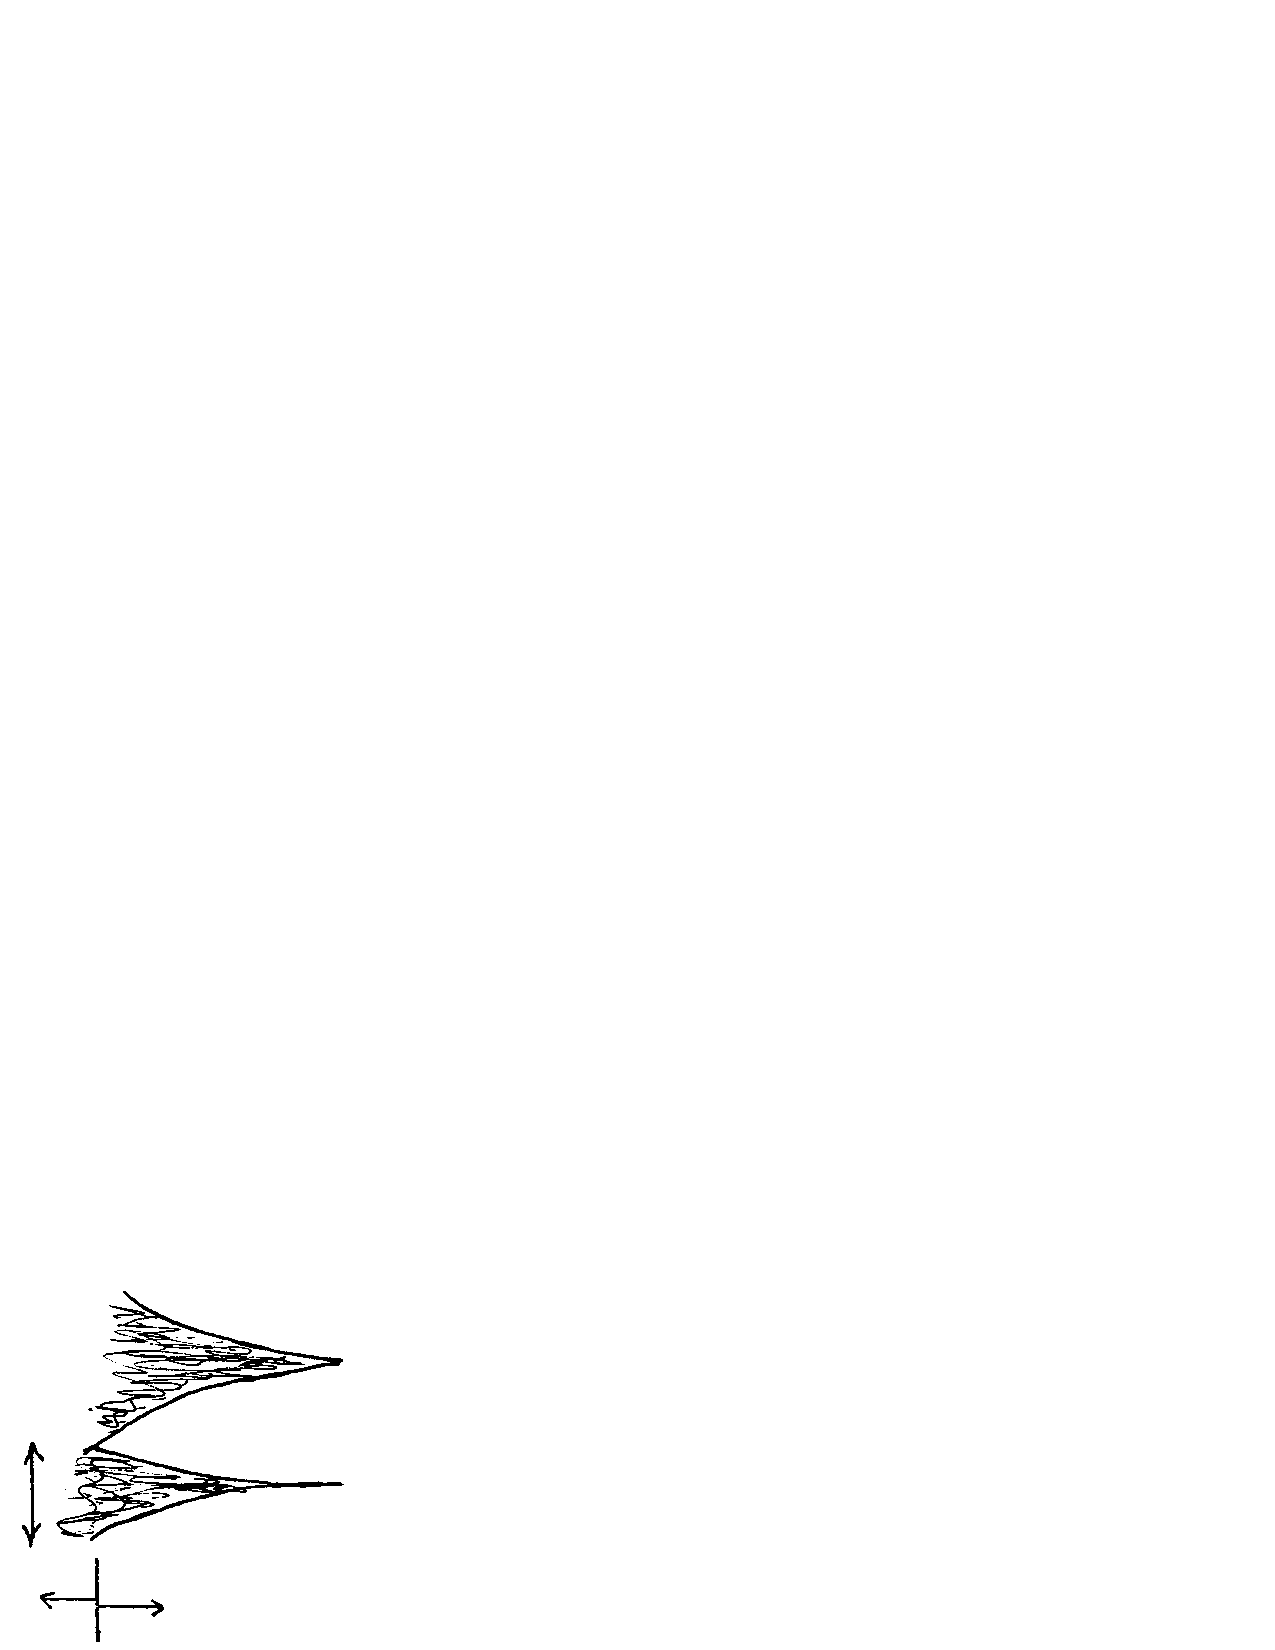
\includegraphics[scale=0.75]{fig14-11}
\caption{The bands for metals of the Mg column. This is just enough to
fill the $3s$ band.  Hence, if distances are large enough the $3p$ and
$3s$ bands would not overlap.  In this case, it would take a finite
energy, the energy gap, to excite an electron and the crystals would
be insulators or semiconductors.  In fact, although these materials
are metals, their conduction properties are consistent with having a
small overlap of the $s$ and $p$ bonds.} 
\label{chap14-fig10}
\end{figure}

The cohesive energy, or total bonding energy per atom, of the Be
column metals are listed in Tables
\ref{chap14-tab3a}--\ref{chap14-tab3b}.  For Mg, Ca, Sr, and Ba, the
bonding energies are comparable, $\sim$40 kcal, but for Be the bonding
energy is 76.5 kcal, nearly twice as large.  This is probably because
first row atoms, such as Be, can make far better lobe bonds than atoms
of this row, as discussed in Chapters 6, 7, and 8.

\begin{table}
\caption{Properties of crystals of Be and Zn 
columns: fcc, hcp, and bcc phases$^c$  }
\label{chap14-tab3a}
\begin{tabular}{cccccccc}\\ \hline
&\multicolumn{2}{c}{Face-Centered Cubic}
&\multicolumn{3}{c}{Hexagonal Closest-Packed}
&\multicolumn{2}{c}{Body-Centered Cubic}\cr
& T & R & T & c/a & R & T & T\cr
& ($^{\circ}$K) & (\AA) & ($^{\circ}$K) & & (\AA) & ($^{\circ}$K) & 
(\AA)\cr

Be & - & - & $\leq$1527 & 1.5680 & 2.225$^i$ & $>$1527 & 2.209\cr
& & & & & 2.236$^i$\cr
Mg & - & - & all$^i$ & 1.6236 & 3.197$^i$ & - & -\cr
& & & & & 3.209$^i$\cr
Ca$^e$ & $\geq 720(\alpha)$ & 3.951$^i$ & $g$ & $g$ & $> 720(\beta)$ & 
3.880\cr
Sr$^d$ & $\leq 830(\alpha)$ & 4.303$^i$ & - & $h$ & $h$ & 
$>830(\gamma)$ & 4.19\cr
Ba$^a$ & - & - & - & - & - & all$^i$ & 4.350$^i$\cr
Ra & - & - & - & - & - & all$^i$ & 4.458$^i$\cr
Zn & - & - & all$^i$ & 1.8561 & 2.664 & - & -\cr
& & & & & 2.912\cr
Cd & - & - & all$^i$ & 1.8855 & 2.979 & - & -\cr
& & & & & 3.293\cr
Hg & all & 3.465$^b$ & - & - & - & - & -\cr
& & 2.993$^b$\cr
\hline
\end{tabular}
\end{table}

\begin{table}
\caption{Properties of crystals of Be and Zn 
columns: temperature and cohesive energy.}
\label{chap14-tab3b}
\begin{tabular}{ccccc}\\ \hline
& $T_{mp}$ & $\Delta H_m$ & $T_{bp}$ & Cohesive Energy 0$^{\circ}$K\cr
& ($^{\circ}$K) & (kcal) & ($^{\circ}$K) & (kcal)\cr
\noalign{\medskip\hrule\medskip}
Be & 1560 & 2.9 & 2745 & 76.5\cr
Mg & 922 & 2.140 & 1363 & 34.7\cr
Ca$^e$ & 1112 & 2.04 & 1757 & 42.5\cr
Sr$^d$ & 1041 & & 1650 & 34.5$^f$\cr
Ba$^a$ & 1002 & 1.85 & 2171 & 43.7\cr
Zn & 692.655 & 1.75 & 1180 & 31.0\cr
Cd & 594.18 & 1.48 & 1040 & 26.73\cr
Hg & 234.28 & 0.5486 & 630 & 14.418\cr
\hline
\end{tabular}\\
$^a$ At 59 kbar pressure, an hexagonal closest-packed structure 
with $R = 3.813$ and 3.901 is stable. 
$^b$ Hg has a rhombohedral structure, A10-type,
corresponding to a distorted face-centered cubic with six nearest-neighbor 
atoms at 2.993 \AA, and six at 3.465 \AA.  A body-centered tetragonal
structure, HgII or BHg, is stable below 79$^{\circ}$K, formed at 
high pressure.
$^c$ Distances are from reference 4b.  Other quantities 
from reference 2.
$^d$ $\beta$Sr with the hexagonal closest-packed structure is now 
known to be a hydride.   $\Delta H_{\alpha \gamma} = (0.191)$ kcal.
$^e$ $\Delta H_{\alpha \beta}$ = 0.22 kcal.
$^f$ Value for $T = 1650^{\circ}$K. 
$^g$ Impure Ca yields a hexagonal closest-packed phase for 
648$^{\circ}$K to 773$^{\circ}$K, and a 
complex phase at 573$^{\circ}$K to 648$^{\circ}$K. 
$^h$ An hexagonal closest-packed phase has been
observed for 486$^{\circ}$K to 894$^{\circ}$K, but may be due to impurities.
$^i$ Bond distances for 25$^{\circ}$C, others are at higher 
temperatures.
\end{table}

\section{The B Column}

The bonding of B$_2$, Al$_1=2$, Ga$_2$, etc., is such that there are many 
orbitals available for bonding to additional atoms,
\begin{equation}
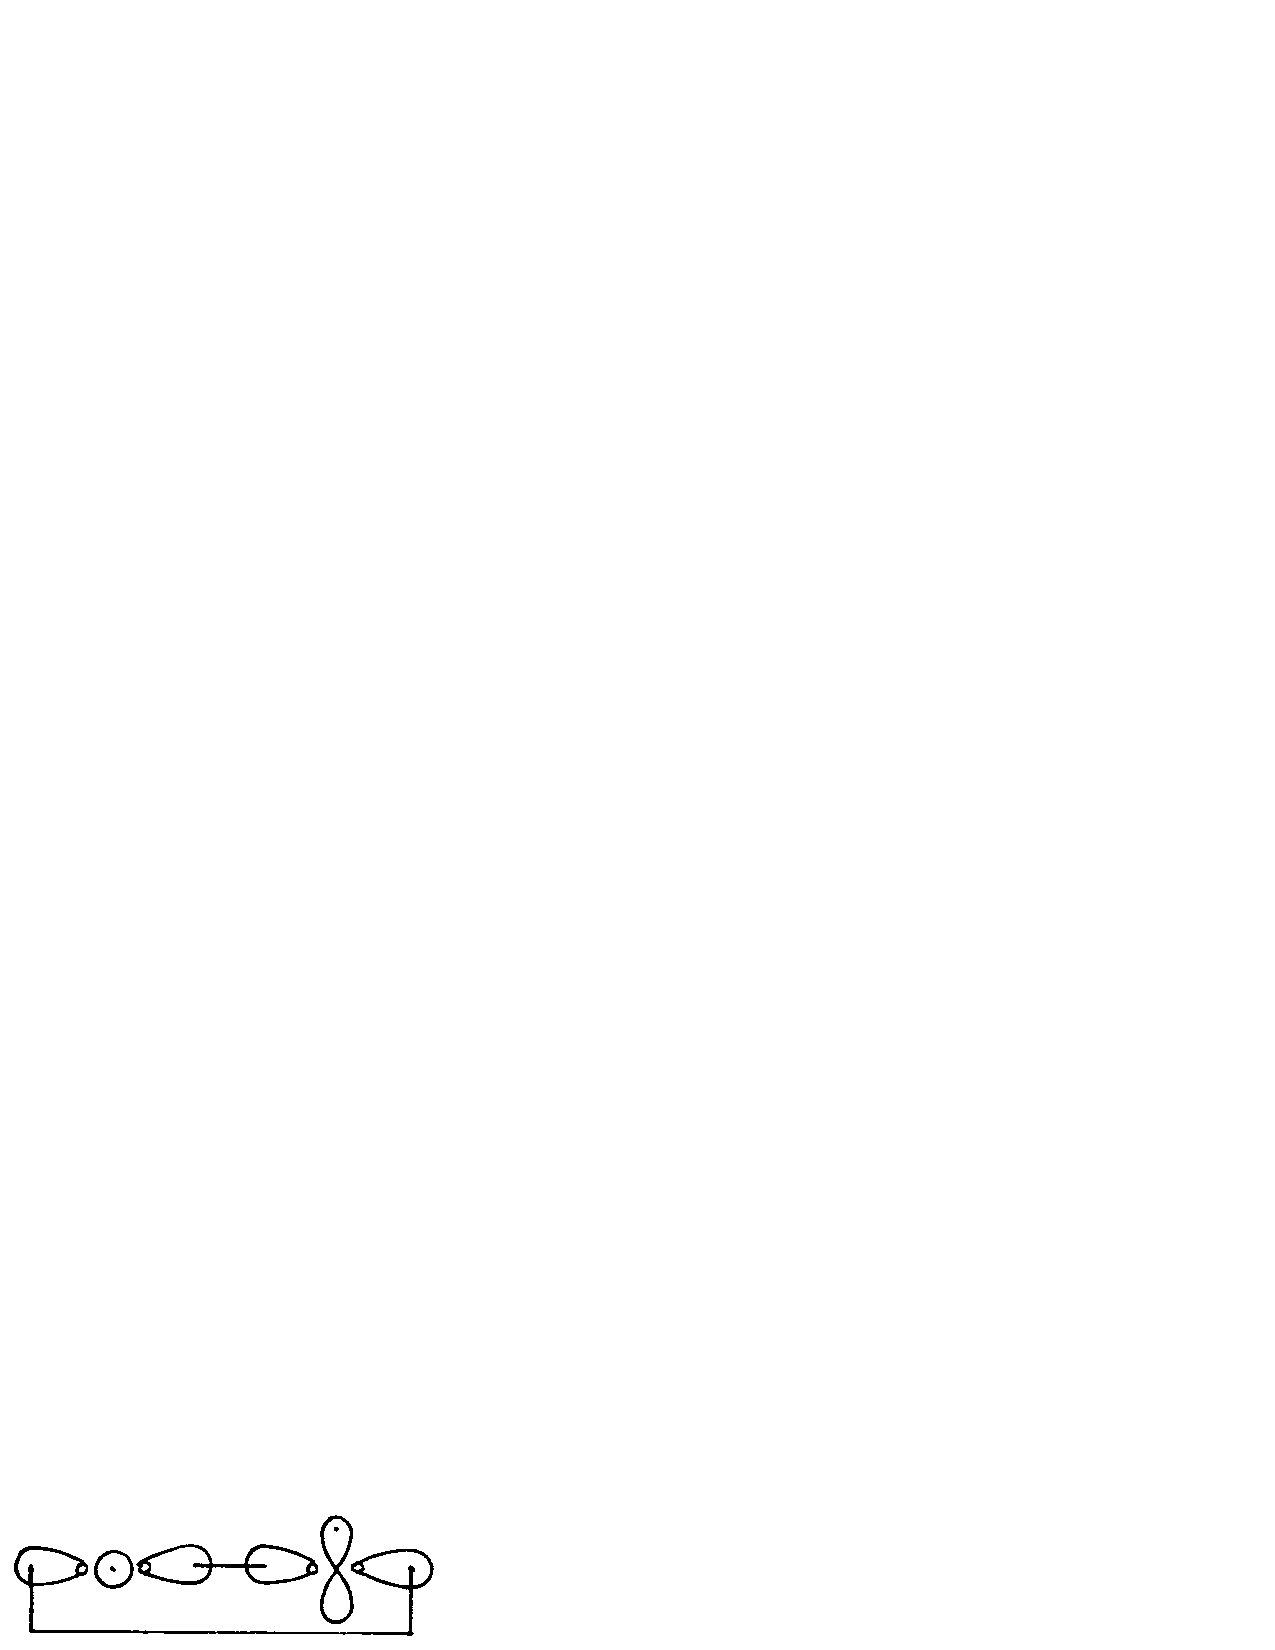
\includegraphics{fig14-12}
\label{chap14-eqno8}
\end{equation}
Indeed a two-dimensional layer of the form
\begin{equation}
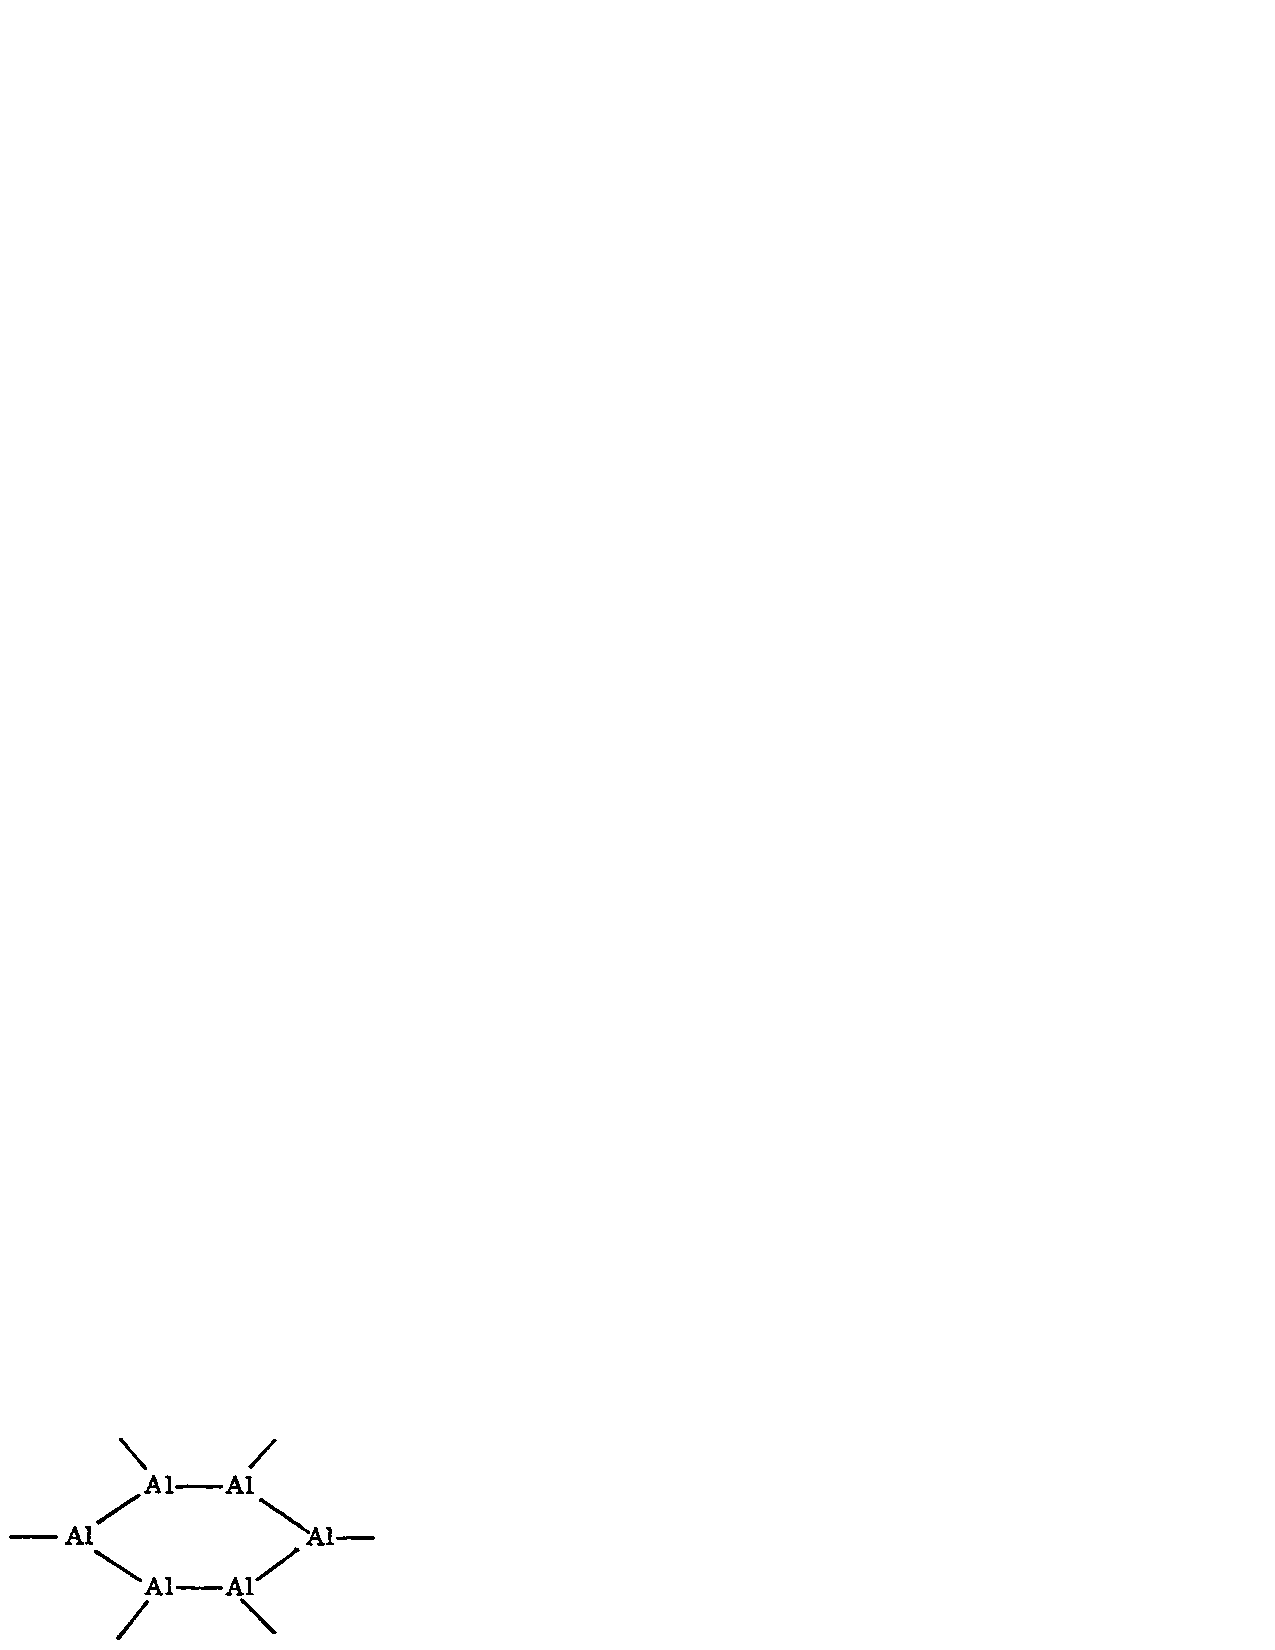
\includegraphics{fig14-13}
\label{chap14-eqno9}
\end{equation}
with all bond orbitals paired, might well be stable under certain 
circumstances.  There is no evidence yet, for such two-dimensional 
networks. The crystal structures of the B column exhibit
no obvious trends. 

\subsection{Boron}

There are three well-characterized forms of B, and many poorly 
characterized forms$^{4a}$:

\begin{description}
\item[$\alpha$] a rhombohedral crystal with twelve atoms per unit 
cell, also denoted R-12 or B$_{12}$
\item[$\beta$] a rhombohedral crystal with 105 atoms per unit cell, 
also denoted R-105 or B$_{105}$ 
\item[$\gamma$] a tetragonal crystal 
with fifty atoms per unit cell, also denoted T-50 or B$_{50}$.
\end{description}

Freezing of molten boron leads to $\beta$, and heating $\alpha$ 
to 1773$^{\circ}$K leads to $\beta$, a black crystal with metallic 
luster.  $\alpha$ and $\gamma$ are obtained by more complicated 
procedures, but $\alpha$ may be the stable form at lower 
temperatures.  $\beta$ may be the stable form above 1373$^{\circ}$K.

$\alpha$B, R-12, consists of nearly regular icosahedra, twelve atoms, 
stacked in a deformed face-centered cubic fashion.  Each atom of an 
icosahedron is bonded at five atoms within the icosahedron.  In addition, 
six are bonded to one atom of an adjacent icosahedron, the linear 
bond, while six are bonded to an atom of each of two icosahedra, the 
triangle bond.  The average bond length within an icosahedron is 1.774 
\AA, ranging from 1.733 to 1.787 \AA, while
the average bond length between clusters is 1.92 \AA, ranging from 1.709 to
2.021 \AA.
	
$\beta$B, R-105, consists of three basic units.  A
is an icosahedron with average internal bond lengths of 1.767 \AA, B 
is an icosahedron with average internal bond lengths of 1.850 \AA, 
and, C is a fused icosahedron, 28 atoms, with average internal bond
lengths of 1.805 \AA.  These units are bonded together with a sprinkling
of external atoms.
	
$\gamma$B, T-50, consists of four nearly regular icosahedra, with an average
internal bond length of 1.806 \AA, ranging from 1.763 to 1.860 \AA, 
bonded together using two extra atoms, each having four bonds.  Each atom 
of an icosahedron is bonded to one external atom, in addition to the five 
within the
icosahedron, and each extra atom is bonded to one atom on each of four
icosahedra. The average bond length is 1.711 \AA.  The external atoms may be 
within another icoshedron or one of the extra atoms.  

At least $\alpha$ and $\gamma$, and probably $\beta$, can be understood 
by assuming that there is a one-electron orbital localized along every bond 
axis. 	As a result, internal bonds within each icosahedron use 30 of the 
36 electrons of each B.  For $\alpha$B, the six linear bonds between 
icosahedra use up three more electrons leaving three electrons for the 
six triangle bonds.  Thus, the triangles end up with 3/2 electron 
each.  For $\gamma$B, putting one electron into each bond axis uses up 
148 electrons of the 150 electrons leaving an excess of two.

\subsection{Aluminum}

On the other hand, aluminum has the face-centered cubic structure at 
all temperatures, $R = 2.864$ \AA.

\subsection{Gallium}

Gallium exhibits a structure with one short bond, 2.465 \AA, to each
atom and six other relatively short bonds, two at 2.700 \AA, two at
2.735 \AA, and two at 2.792 \AA.$^{4b}$ The structure can be viewed as
follows.  Take a closest-packed layer and distort it so that half the
atoms move down, D, and half move up, U, as indicated below:
\begin{equation}
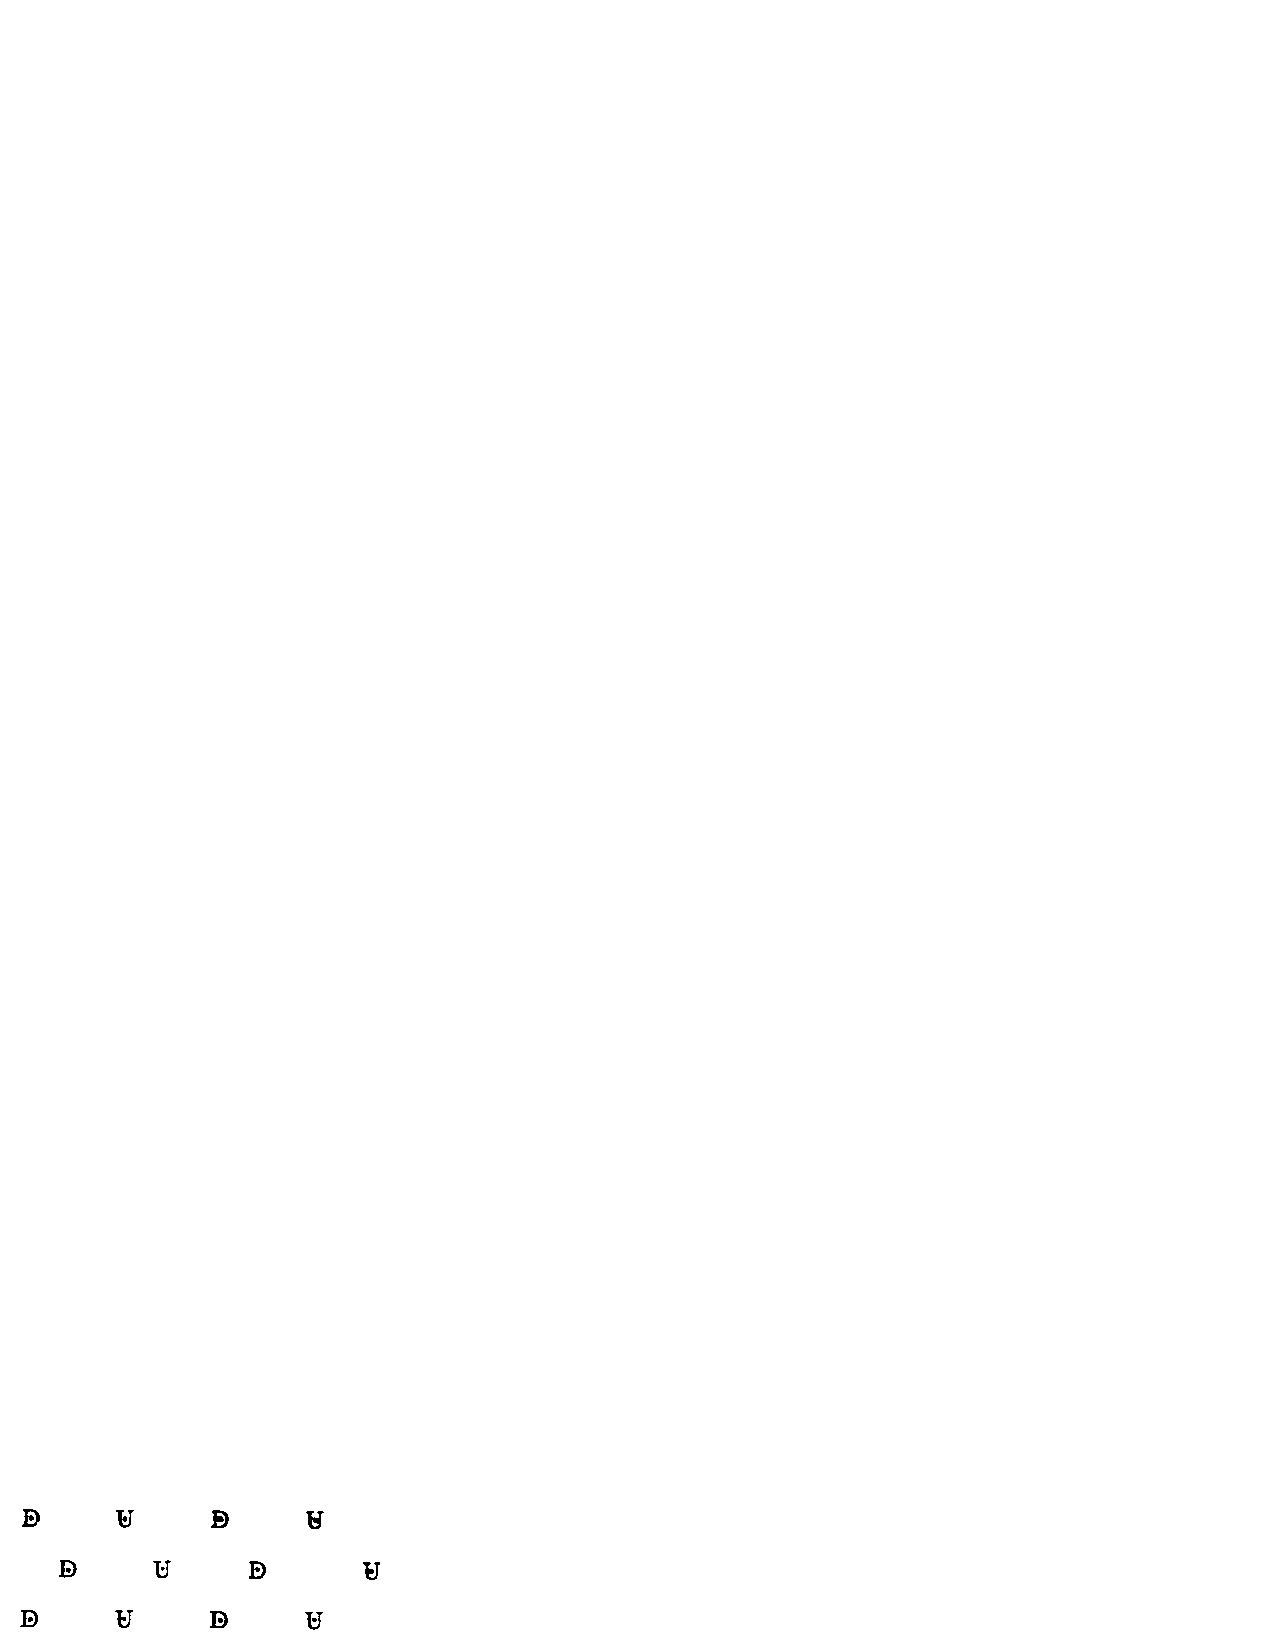
\includegraphics{fig14-14}
\label{chap14-eqno10}
\end{equation}
Within this plane, each of these atoms has two bonds at 2.700 \AA, two at
2.735 \AA, and two at 2.792 \AA.  These layers are stacked so that each D atom 
of one layer is bonded to one U atom of the layer below, bond distance 
2.465 \AA.  This could be rationalized by orienting the orbitals of Ga as
\begin{equation}
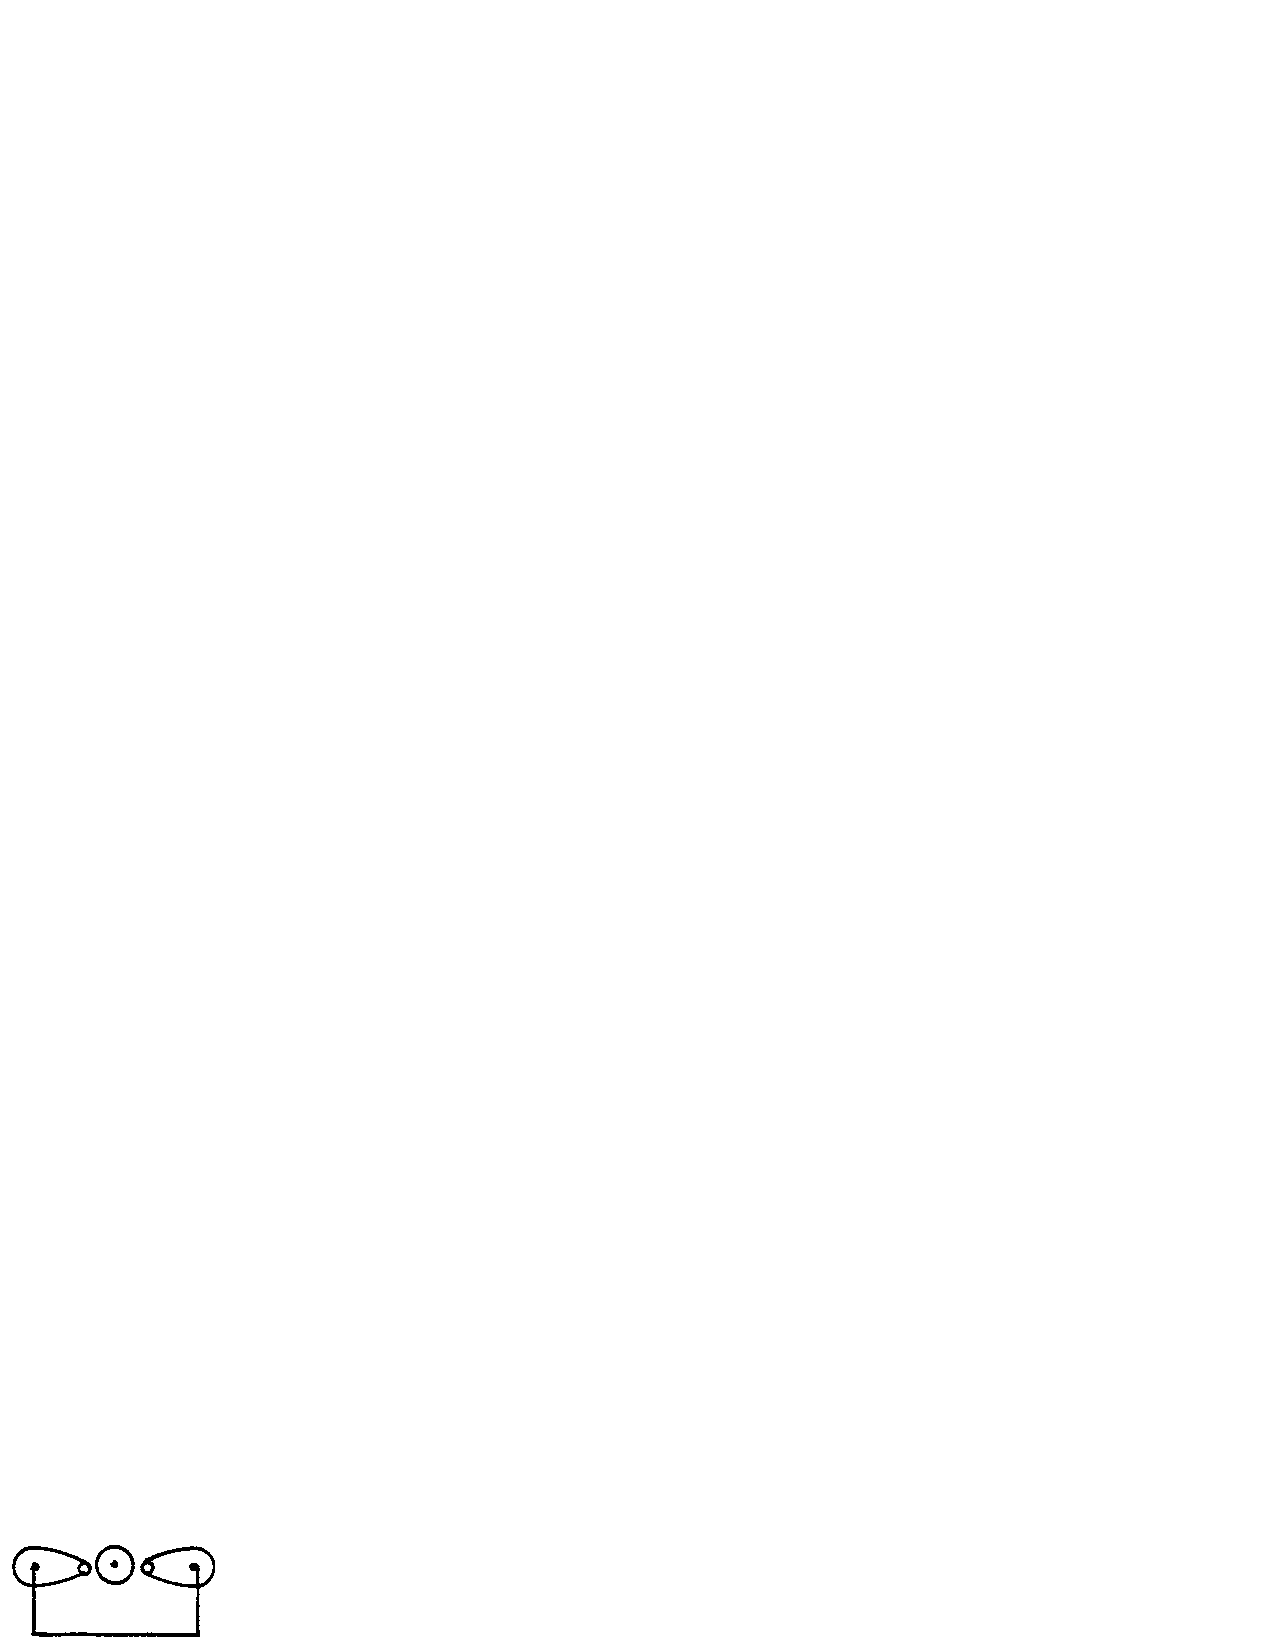
\includegraphics{fig14-15}
\label{chap14-eqno11}
\end{equation}
with the unpaired electrons in the $z$ direction.  Then, within the
$xy$ layer we can make bonds as in equation (\ref{chap14-eqno6}),
leading to a closest-packed layer.  The orbital in the $z$ direction
can bond either to a layer above or below the current layer.
Alternating the bond to one side or the other for adjacent atoms,
leads then to equation (\ref{chap14-eqno9}), with half the atoms
puckered up and the other half down.

\subsection{Indium}

Indium has a structure that is a slight distortion of face-centered 
cubic, with four bonds of 3.251 \AA, and eight of 3.373 \AA.$^3$

\subsection{Thallium}

Thallium exhibits the hexagonal closest-packed structure, $\alpha$,
below 507$^{\circ}$K, and the body-centered cubic structure, $\beta$,
above 507$^{\circ}$K.$^2$ The bond distances are 3.408 and 3.457 \AA\
for hexagonal closest-packed and 3.362 for body-centered cubic. The
problem with obtaining a qualitative understanding of why one
structure forms for one element and another structure for a similar
element, can be illustrated here.  The difference in enthalpy between
the hexagonal closest-packed and the body-centered cubic forms of
thallium is 0.090 kcal.$^2$ Thus, the factors determining which
structure is stable may involve very subtle factors indeed.

\subsection{Properties}

Some properties are summarized in Table \ref{chap14-tab4}.  Once
again, the first-row compound, B, is about a factor of two more
strongly bound than the others.  Again, this is probably due to the
strong lobe bonds formed by first row atoms.  There is a gradual
decrease in bond strength as we proceed down the periodic table. This
trend is reflected in the boiling points, but there are some
fluctuations in melting temperatures.

\begin{table}
\caption{Crystalline properties of the B column.$^a$}
\label{chap14-tab4}
\begin{tabular}{cccccc}\\ \hline
& & $T_{mp}$ & $\Delta H_m$ & $T_{bp}$ & Cohesive\cr
& & & & & Energy\cr
& & ($^{\circ}$K) & (kcal) & ($^{\circ}$K) & (kcal)\cr
\noalign{\medskip\hrule\medskip}
B & B$_{12}$, $T < 1373^{\circ}$K & 2300 & 12.0 & 4275 & 135.3\cr
& B$_{105}$, $T > 1373^{\circ}$K\cr
Al & face-centered cubic, all $T$ & 933.25 & 2.58 & 2793 & 78.1\cr
Ga & orthorhombic, all $T$ & 302.90 & 1.336 & 2478 & 64.8\cr
In & tetragonal, all $T$ & 429.76 & 0.780 & 2346 & 58.1\cr
Tl & $\alpha$ hexagonal closest-packed, $T < 507^{\circ}$K & 577 & 
0.99 & 1746 & 43.4\cr
& $\beta$ body-centered cubic, $T > 507^{\circ}$K$^b$\cr
\hline
\end{tabular}\\
$^a$ Reference 2, unless otherwise noted.
$^b$ $\Delta H_{\alpha \beta} =$ 0.090 kcal.
\end{table}

\section{Group IV Metals}

For temperatures below 286.2$^{\circ}$K, the stable form of Sn has the
tetrahedral diamond structure, referred to as gray Sn or $\alpha$Sn.
However, at higher temperatures, the stable form of Sn is metallic,
white Sn or $\beta$Sn, with a crystal structure, type A5, in which
each Sn has six near neighbors rather than four, as shown in Figure
\ref{chap14-fig11}.  This structure can be viewed as follows:

\begin{figure}
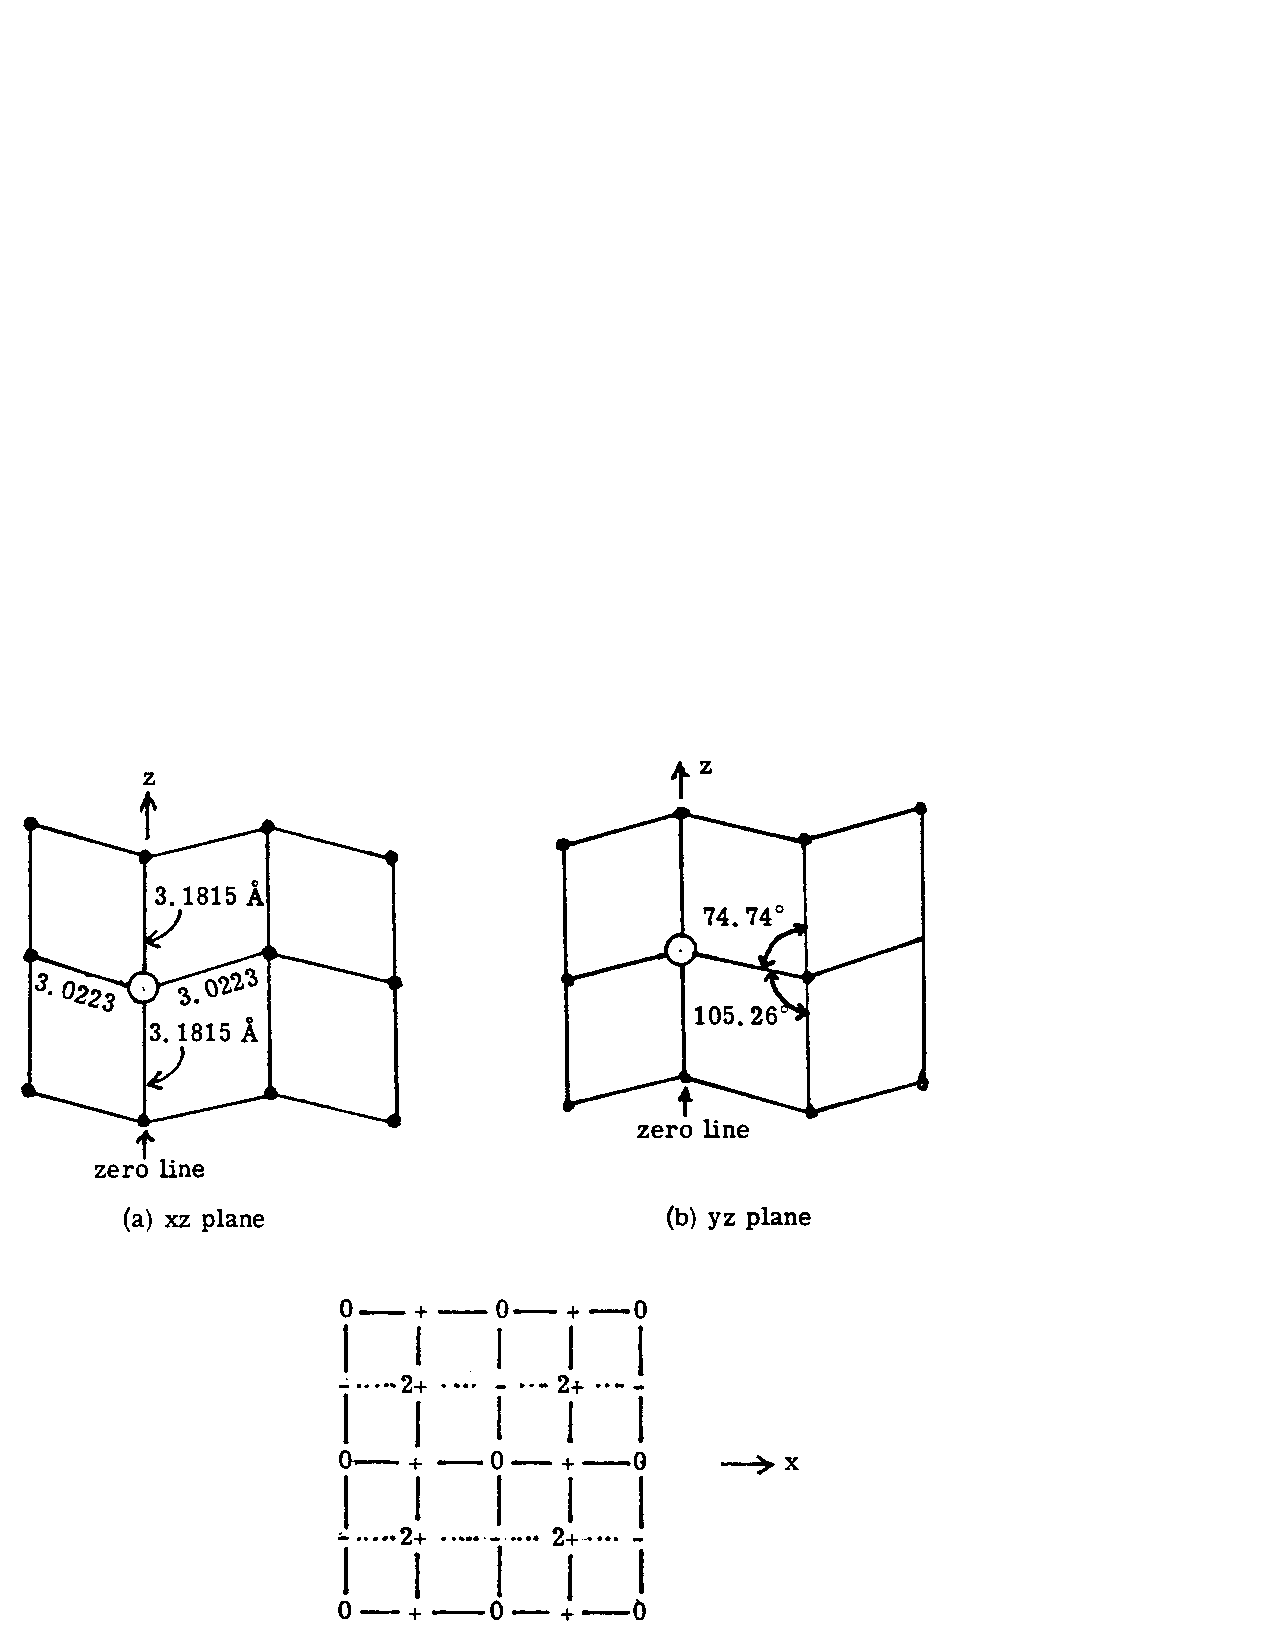
\includegraphics[scale=0.75]{fig14-16}
\caption{The structure of $\beta-$Sn (white Sn) is shown.  
(a) on the $xz$ plane, (b) on the $yx$ plane, and (c) on the $xy$
plane.  In (c) the solid lines connect one two-dimensional layer, and
0, $\pm$, $\pm 2$, etc., indicating height in $z$ direction; dotted
lines indicate connections of different layers.}
\label{chap14-fig11}
\end{figure}

Start with a square net of Sn atoms and distort as in Figure
\ref{chap14-fig11}(c).  Solid lines connect bonds of the layer, so
that the four bonds from a squashed tetrahedron at each atom, and
dotted lines indicate equivalent bonds connecting other layers.  Then
add layers above and below with new atoms in the $\pm z$ direction.
Four neighbors are at 3.022 \AA, and two are at 3.182 \AA, with bond
angles of 75$^{\circ}$, 94$^{\circ}$, and 105$^{\circ}$.  In
comparison, for gray Sn the four bond lengths are 2.810 \AA.  At the
transition temperature, the enthalpy of gray Sn is 0.47 kcal lower
than that of white Sn.

At high pressures, both Si and Ge also convert to the white Sn
structure, above 195 kbar for Si and above 120 kbar for Ge.  The bond
distances are as in Table \ref{chap14-tab5}.  Since the white tin
structure has higher coordination, it is reasonable that it becomes
relatively more stable at higher pressures.

Similar III-V structures with the tetrahedral diamond-like structure,
sphalerite, such as InSb, GaSb, AlSb, etc., exhibit a white tin-like
structure at high pressure.  Crystalline lead has the face-centered
cubic structure with a bond distance of 3.5003 $\pm$ 0.004.  The
properties of these metals are given in \ref{chap11-tab3}.


\begin{table}
\caption{Bond distances for white Sn structures.}
\label{chap14-tab5}
\begin{tabular}{cccc}\\ \hline
& Four & Two\cr
\noalign{\medskip\hrule\medskip}
$\beta$ Si & 2.430 & 2.585 & above 195 kbar\cr
$\beta$ Ge & 2.533 & 2.692 & above 120 kbar\cr
$\beta$ Sn & 3.022 & 3.182 & 1 atm.\cr
\hline
\end{tabular}
\end{table}
